%% LaTeX2e class for student theses
%% thesis.tex
%% 
%% Karlsruhe Institute of Technology
%% Institute for Program Structures and Data Organization
%% Chair for Software Design and Quality (SDQ)
%%
%% Dr.-Ing. Erik Burger
%% burger@kit.edu
%%
%% See https://sdqweb.ipd.kit.edu/wiki/Dokumentvorlagen
%%
%% Version 1.3.5, 2020-06-26

%% Available page modes: oneside, twoside
%% Available languages: english, ngerman
%% Available modes: draft, final (see README)
\documentclass[twoside, english]{sdqthesis}

% \usepackage{ amssymb }
\usepackage{listings}
\usepackage{xargs}
\usepackage{simplebnf}
\usepackage{numprint}
\usepackage{ amsmath }
\usepackage{mathpartir}
\usepackage{minted}
\usemintedstyle{colorful}
% \usepackage{amsthm}
% \usepackage{csquotes}
\usepackage{ stmaryrd }
\usepackage{stackengine,scalerel}
\usepackage{mathtools}
\usepackage[nameinlink]{cleveref}
\usepackage{xparse}
% \usepackage[scaled=.78]{beramono}
% \usepackage[scaled=.92]{sourcesanspro}

% \usepackage{tgcursor}
% \usepackage{cascadia-code}
% \setmonofont[]{cascadia}

% \usepackage{fontspec}
% \usepackage[zerostyle=d]{newtxtt}
% \usepackage[scaled=.5,proportional,lightcondensed]{zlmtt}
% \usepackage{fontspec}
% \setmonofont{Fira Code}[
%   Contextuals=Alternate  % Activate the calt feature
% ]
% \setmonofont{Latin Modern 
% \usepackage{nimbusmononarrow}
% \usepackage[nomath]{lmodern}

% \setmonofont[scaled=0.8]{Comic Mono}
% \setmonofont{Noto Sans Mono}
\usepackage[scale=0.87]{sourcecodepro}
% \usepackage{inconsolata}

% % Looks good:
% \usepackage{DejaVuSansMono}
% \setmonofont{DejaVu Sans Mono}
% \usepackage[]{lmodern}

\usepackage[]{todo}
% \usepackage[colorinlistoftodos,prependcaption,textsize=tiny]{todonotes}

% \newcommandx{\unsure}[2][1=]{\todo[linecolor=red,backgroundcolor=red!25,bordercolor=red,#1]{#2}}
% \newcommandx{\change}[2][1=]{\todo[linecolor=blue,backgroundcolor=blue!25,bordercolor=blue,#1]{#2}}
% \newcommandx{\info}[2][1=]{\todo[linecolor=OliveGreen,backgroundcolor=OliveGreen!25,bordercolor=OliveGreen,#1]{#2}}
% \newcommandx{\improvement}[2][1=]{\todo[linecolor=Plum,backgroundcolor=Plum!25,bordercolor=Plum,#1]{#2}}

% \newcommand{\code}[1]{\texttt{#1}} 

\newcommand{\mtext}[1]{$\text{#1}$}
\newcommand{\tuple}[2]{\langle #1 \mid #2 \rangle}
\newcommand{\bbracket}[1]{\llbracket #1 \rrbracket}
\newcommand{\tr}[0]{\triangleright}

\newcommand{\ccolon}[0]{: }
\newcommand{\cmid}[0]{| }
\newcommand{\cdisj}[0]{|| }

\DeclareMathOperator{\rref}{ref}
\DeclareMathOperator{\dom}{dom}
\DeclareMathOperator{\img}{img}

\makeatletter
\NewDocumentCommand{\rulelabel}{m}{%
  \begingroup
  \protected@edef\@currentlabelname{Rule}%
  \protected@edef\cref@currentlabel{%
    [][][]%
    #1
  }
  \label[typerule]{rule:#1}%
  \endgroup  
}
\makeatother

\crefname{typerule}{}{}
\Crefname{typerule}{}{}

% \newcommand{\tyrule}[4]{\ensuremath{
%   \infer
% }}



\newtheorem{theorem}{Theorem}[section]
\newtheorem{corollary}{Corollary}[theorem]
\newtheorem{lemma}[theorem]{Lemma}
\theoremstyle{definition}
\newtheorem{definition}[theorem]{Definition}


%% ---------------------------------
%% | Information about the thesis  |
%% ---------------------------------

%% Name of the author
\author{Carsten Csiky}

%% Title (and possibly subtitle) of the thesis
\title{LiquidRust: Refinement Types for Imperative Languages with Ownership}

%% Type of the thesis 
\thesistype{Master's Thesis}

%% Change the institute here, ``IPD'' is default
\myinstitute{Institute of Theoretical Informatics (ITI)}

%% You can put a logo in the ``logos'' directory and include it here
%% instead of the SDQ logo
% \grouplogo{myfile}
%% Alternatively, you can disable the group logo
\nogrouplogo

%% The reviewers are the professors that grade your thesis
\reviewerone{Prof. Dr. Bernhard Beckert}
% \reviewertwo{}

%% The advisors are PhDs or Postdocs
\advisorone{Dr. Mattias Ulbrich}
%% The second advisor can be omitted
\advisortwo{Sebastian Graf, M.Sc.}
\advisorthree{Florian Lanzinger, M.Sc}

%% Please enter the start end end time of your thesis
\editingtime{4.4.2022}{4.10.2022}

\settitle

%% --------------------------------
%% | Settings for word separation |
%% --------------------------------

%% Describe separation hints here.
%% For more details, see 
%% http://en.wikibooks.org/wiki/LaTeX/Text_Formatting#Hyphenation
\hyphenation{
% me-ta-mo-del
}

%% --------------------------------
%% | Bibliography                 |
%% --------------------------------

%% Use biber instead of BibTeX, see README
\usepackage[citestyle=numeric,style=numeric,backend=biber]{biblatex}
\addbibresource{thesis.bib}


%% ====================================
%% ====================================
%% ||                                ||
%% || Beginning of the main document ||
%% ||                                ||
%% ====================================
%% ====================================
\begin{document}

%% Set PDF metadata
\setpdf

%% Set the title
\maketitle

%% The Preamble begins here
\frontmatter

%% LaTeX2e class for student theses: Declaration of independent work
%% sections/declaration.tex
%% 
%% Karlsruhe Institute of Technology
%% Institute for Program Structures and Data Organization
%% Chair for Software Design and Quality (SDQ)
%%
%% Dr.-Ing. Erik Burger
%% burger@kit.edu
%%
%% Version 1.3.5, 2020-06-26

\thispagestyle{empty}
\null\vfill
\noindent\hbox to \textwidth{\hrulefill} 
\iflanguage{english}{I declare that I have developed and written the enclosed
thesis completely by myself, and have not used sources or means without
declaration in the text.}%
{Ich versichere wahrheitsgemäß, die Arbeit
selbstständig angefertigt, alle benutzten Hilfsmittel vollständig und genau
angegeben und alles kenntlich gemacht zu haben, was aus Arbeiten anderer
unverändert oder mit Änderungen entnommen wurde.}
 
 
%% ---------------------------------------------
%% | Replace PLACE and DATE with actual values |
%% ---------------------------------------------
\textbf{Karlsruhe, 4.10.2022}
\vspace{1.5cm}
 
\dotfill\hspace*{8.0cm}\\
\hspace*{2cm}(\theauthor) 
\cleardoublepage

\setcounter{page}{1}
\pagenumbering{roman}

%% ----------------
%% |   Abstract   |
%% ----------------
 
%% For theses written in English, an abstract both in English
%% and German is mandatory.
%%
%% For theses written in German, a German abstract is sufficient.
%%
%% The text is included from the following files:
%% - sections/abstract

\includeabstract

%% ------------------------
%% |   Table of Contents  |
%% ------------------------
\tableofcontents

\listoffigures
\listoftables
\listoflistings

%% -----------------
%% |   Main part   |
%% -----------------

\mainmatter

\iftrue % shorten
\chapter{Introduction}


% With increasing reliance on increasingly complex software, ensuring correctness of programs is a vital concern to software development.
With increasing amount and reliance on software, ensuring the correctness of programs is a vital concern for the future of software development.
Although research in this area has made good progress, most approaches are not accessible enough for general adoption by the developers. Especially in light of a predicted shortage of developers\cite{breaux_2021_2021-1}, it is not sufficient to require developers to undergo year-long training in specialized and complex verification methods to ensure the correctness of their software. It is therefore crucial to integrate with their existing tooling and workflows to ensure the future high quality of software.
One avenue for improving accessability for functional verification is extending the expressiveness of the type system to cover more of the correctness properties.
Using type systems for correctness was traditionally prevalent in purely functional languages where evolving states are often represented by evolving types, offering approachable and gradual adoption of verification methods. Tracing evolving states in the type system would be especially useful for languages with mutability, since substantial parts of the behaviour of the program is expressed as mutation of state. In particular Rust seems like a promising target language, because mutability is already tracked precisely and thus promising functional verification for relatively minimal effort on the programmer's part.

The goal of the thesis is to show that Refinement Types can be idiomatically adapted to languages with unique mutable references. The type system presented in this thesis enables gradual adoption of lightweight verification methods in mutable languages.

%In case implementing these translations could not be completed, the use cases will be transformed manually.
The type system is sound and effective in the identified use-cases.
%In addition, a description of the syntax and semantics of the constructs, that will extend Rust's type system, will be provided as well as justification for their soundness. 
A feasibility study on minimal examples of challenging use cases shows how useful the proposed verification system is. 
%For use cases that could not be covered by the proposed additions, the reason will be investigated.

Specifying or verifying complete Rust modules or the entire Rust language is not the goal of the thesis. In particular \code{unsafe} Rust will not be taken into account in specification nor implementation. Implementing Liquid Type inference is also not a goal of the thesis.

The accompanying implementation extends the Rust compiler, enables automatic parsing of the refinement type language and automated type checking of a subset of Rust, as well as limited inference and error reporting. 
% The thesis also gives a description of the syntax and semantics of the subset of Rust as well as the refinement type system.

The main contributions of this thesis are:
\begin{enumerate}
  \item Automatic empirical analysis of the usage of mutability and unsafe in Rust using syntactic information
  \item Extension to the Rust type system to allow for refinement type specifications
  \item Description and implementation of a type checker for the introduced type system
  \item Evaluation of the type system on minimal benchmarks
\end{enumerate}

The thesis if structured as follows: 
\Cref{ch:foundations} will give an overview of the foundation the thesis build upon.
Thereafter in \cref{ch:analysis} an empirical analysis of \code{unsafe} and mutability uses is performed to gain an understanding of how Rust is used.
\Cref{ch:language} defines the subset of Rust, that will be the basis for the type system.
Next \cref{ch:type-system} explains the actual type system and type checking, as well as justifying its correctness, followed by chapter \cref{ch:implementation}, which will provide additional information about how the type system was implemented.
The implementation will then be tested on minimal benchmarks in \cref{ch:evaluation}.
\Cref{ch:related-work} reports on related work and alternative approaches.
Finally \cref{ch:conclusion} concludes the thesis and gives an overview over possible future work.

\chapter{Foundations} \label{ch:foundations}

We start by giving a basic overview over the fundamental concepts, that are relevant for our work.
The semantics of our subset of Rust are discussed in \cref{ch:language}.

\section{Refinement Types}

The type system, that this thesis will adapt, is based on the Refinement Type system described by Vazou et al. \cite{vazou_abstract_2013} and Rondon et al. \cite{rondon_liquid_2008}. 
The central idea of Refinement Types is adding predicates to a language's type: For example, a type \code{i32} might be refined with the predicate $v > 0$. The refined type is written as $\left\{ v : \text{i32} \mid v > 0 \right\}$. In terms of semantics this means, that any inhabitant of that type must also satisfy the predicate. 

The notion of refinements is embedded into the base language using subtyping: A refined type $\tau$ is a subtype of $\tau'$ if $\tau$'s predicate implies the predicate of $\tau'$ (in the current typing context $\Gamma$).
As is common with subtyping systems, the subtype can then be used in the place where the super type is expected.
The following rule shows how subtyping is handled by Liquid types \cite[p. 6]{rondon_liquid_2008}:

\begin{equation*}
  \inferrule*
    {\text{SMT-Valid}(\llbracket \Gamma \rrbracket \wedge \llbracket e_1 \rrbracket \Rightarrow \llbracket e_2 \rrbracket)}
    {\Gamma \vdash \left\{ v : b \mid e_1 \right\} \preceq \left\{ v: b \mid e_2 \right\}}
\end{equation*}

Refinement Types are related to dependent types, distinguished by the limited expressiveness of the type. Refinement types trade off expressiveness for automatic type checking. Allowed formulas are chosen from a SMT decidable logic. 
Rondon et al. \cite{rondon_liquid_2008} chose the EUFA as the logic fragment, meaning a propositionaly logic with the theories of equality, uninterpreted functions and linear arithmetic.


\section{Rust}

The Rust programming language \cite{matsakis_rust_2014} is a multi-paradigm systems programming language, originally developed by Graydon Hoare at Mozilla Research.
Even though Rust is quite young, the first stable release published in 2015, it has attracted interest in a wide area of applications and organization. It is used everywhere from Volvo building embedded software for cars \cite{foufas_why_2022} to Western Digital implementing a NVMe driver for Linux in Rust \cite{larabel_lpc_2022} and of course the Rust compiler it self.
It draws inspiration from functional and imperative programming languages. The core forms a set of features usually found in functional programming languages: Functions, closures, algebraic data types, type classes (called traits in Rust) and pattern matching, immutability are all common place in Rust.
However, Rust is also influenced by C: Rust extends its ML base with optional mutability of data and references and manual memory management. Many design decisions of Rust can be explained by Rust's ambitions to offer safe and clear ML-like abstractions without compromising on performance compared to C.
For example, Rust elected to use manual memory management like C, which guarantees faster and predictable execution times when compared to garbage collection. Crucial, Rust does not compromise on safety to accomplish this: To this end, Rust incorporates the notion of affine types into its type system (called \textit{ownership system} in Rust). This additional type system guarantees, 
Inspired by research language Cyclone introduced by Grossman et al. \cite{grossman_region-based_nodate}, this type system guarantees the absence of memory errors.
% The Rust programming language is designed to offer tight control over the amount of mutability and what it mutation can effect. 
Rust also offers a special language subset called \code{unsafe} Rust, which deactivates the static ownership checking and places the responsibility of ensuring memory safety on the programmer, analogous to C. \code{unsafe} Rust is used to provide low-level primitives, that expose a safe interface, that can be used in safe Rust. From here on out, we will focus on safe Rust.

Among other things, the ownership system is used to handle memory management, safe concurrency and simplifies reasoning about program behaviour.
The next paragraph will explain how the ownership system works.

\paragraph{Aliasing XOR Mutabillity}

The ownership system is an implementation of affine types. It uniquely associates each memory object with an owner. 
The owner of a Rust object is the binding, that is responsible for freeing the object. In the listing \ref{lst:ownership-transfer}, first \code{a} is the owner of the \code{User} object. An object may only be used once, at which point it is consumed and ownership is transferred to its new binding. In the example \code{greet(user)} uses \code{a} and transferring ownership to \code{greet}. At the end of \code{greet}, there is no new owner, as a result the user object is freed.

\begin{listing}[ht]
  \begin{minted}[fontsize=\footnotesize, texcomments]{rust}
    struct User { name: String, age: u32 }

    fn greet(user: User) -> String { // \code{greet} takes ownership for \code{user}
      format!("Hi {}", user.name)
    } // End of scope: Owned value \code{user} is dropped
    ...
    let a = User { name: "Alice", age: 25 };
    let result = greet(a); // Transfer ownership of \code{user} to \code{greet}
    println!(a.name); // error: use of moved value `a`
  \end{minted}
  \caption{Example demonstrating the Ownership System: \code{greet(a)} transfers ownership of \code{a} to \code{greet}}
  \label{lst:ownership-transfer}
\end{listing}

On closer inspection, handing over the ownership of \code{a} to \code{greet} is not sensible: \code{greet} just needs to read the value, but should not take ownership of \code{a}. 
For that purpose, Rust offers a different kind of value transfer called \textit{references}, which have similar execution semantics to pointers. Because creating a reference does not transfer the ownership of the pointee, is is called a \textit{borrow}. Listing \ref{lst:ownership-immut-borrow} rephrases \code{greet} to only take a borrow of the user, instead of taking ownership. Because \code{user} is not owned by \code{greet}, it is not permitted to extract \code{user.name} (of Type \code{String}), instead only borrows to the name are allowed. 

\begin{listing}[ht]
  \begin{minted}[fontsize=\footnotesize, texcomments]{rust}
    fn greet(user: &User) -> String { // \code{greet} borrows \code{user}
      let name_ref : &String = &user.name; // borrow \code{name} from \code{user}
      format!("Hi {}", name_ref)
    } // End of scope: The borrows are dropped, but the user object is not
    ...
    let a = User { name: "Alice", age: 25 };
    let result = greet(&a); // Lend \code{a} to \code{greet}
    println!(a.name); // No error
  \end{minted}
  \caption{Example demonstrating borrowing: \code{greet(\&a)} lends \code{a} to \code{greet}}
  \label{lst:ownership-immut-borrow}
\end{listing}

Borrowing, just like pointers, entail the risk of dangling pointers. Rust protects from this risk, by tracking the lifetimes (i.e. the required duration, where a reference must be valid) of objects. While interesting in its own right, it is not relevant for this thesis.



Mutable references can exacerbate the problem, which leads to the key insight of Rust: 
Memory unsafety can arise from the mere presence of two references where at least one is mutable.
Thus, Rust ensures, that for every variable at every point during the execution, that variable can either aliased or mutable, but never both at the same time. 
\Cref{lst:ownership-mut-borrow} demonstrates that Rust will not accept a problem where aliased and mutable access is possible at a time. To resolve the issue, the mutable reference should be borrows after the call to \code{greet}.


\begin{listing}[ht]
  \begin{minted}[fontsize=\footnotesize, texcomments]{rust}
    fn age(user: &mut User) {
      (*user).age = user.age + 1;
    }
    ...
    let a = User { name: "Alice", age: 25 };
    let b = &a;
    let c = &mut a; // error: cannot borrow `a` as mutable because it is also borrowed as immutable
    age(c);
    let result = greet(&b); // Lend \code{a} to \code{greet}
    println!(a.name);
  \end{minted}
  \caption{Example demonstrating mutable borrowing: \code{age(a)} needs a mutable borrow of user to increase the age, but \code{a} is borrows immutably, which is forbidden}
  \label{lst:ownership-mut-borrow}
\end{listing}

In conclusion ownership makes both aliasing as well as mutability quite tame:
If a variable is aliased, it must be immutable and as a result, represents just a value (like in pure functional languages).
If a variable is mutable, it can not be aliased and as a result, any effect of the mutation is well known and locally visible.
Although the ownership system was originally introduced to allow for safe, manual memory management, it turned out to be useful for other problems as well: For example concurrency, hardware access and automated reasoning all profit from the strong guarantees of safe Rust. The consequences for the latter will be explained in the next subsection.

% Rust accomplishes this by introducing three types of access permissions for a variable, which are associated with every scope\footnote{In modern Rust, this model was generalized to cover more cases, but the idea is still valid}:
% \begin{enumerate}
%   \item The scope \textit{owns} the variable. This guarantees, that no other scope has access to any part of the variable and allows the scope to create references to (part of) the variable. The owner is responsible for freeing the object, which generally happens once the scope is left.
%   \item The scope (immutably) \textit{borrows} the variable. This guarantees, that as long as the variable is used, its \textit{value will not change} and allows the scope to further lend the variable to other scoped.
%   \item The scope \textit{mutably borrows} the variable. This guarantees, that there are no other active references to any part of the memory of the variable.
% \end{enumerate}

% A value may at most be used once, at which point the old variable can no longer be accessed and the new value becomes the owner. This process is called ownership transfer. 

% A consequence of these rules it, that at any time, every piece of memory has a unique and compile-time known owner. There are no reference cycles.


\subsection{Insights into Rust as a Verification Target}

Rust justifies a new approach to verification, because it is possible to take advantage of guarantees provided by Rust's ownership system. 

% Rust is split into two languages: safe and unsafe Rust. Like most type systems, Rust's type and ownership system is conservative, meaning any (safe) Rust program that type checks, will not crash due to memory safety or type errors. Unsafe Rust gives the programmer the ability to expand the programs accepted by Rust outside that known-safe subset.


Rust features a few exceptional design decisions that profoundly influence the design of verification systems for it. The following paragraphs will elaborate on this.


\paragraph*{Opaque Generics} Rust does not provide a way to check a generic parameter for its instantiation. This means that we cannot extract any additional information from a generic parameter \code{T}. A function from \code{T} to \code{T} can therefor only be the identity function.
Wadler \cite{wadler_theorems_1989} shows, that it is possible to derive facts about the behaviour of such polymorphic functions.

In contrast, languages with instance-of-checks allow an implementation of a polymorphic function to distinguish between different instances of the generic parameter, precluding this extensive reasoning.

\paragraph*{Explicit Mutable Access} A consequence of the ownership rules is, that a function can only mutate (part of) the state, that is passed to it as a parameter. There is no global state and there is no implicit access to an object instance. Thus any intention of mutating state must already be expressed in the function signature, which makes the specification of this mutation quite natural.

\paragraph*{Minimal subtyping} In contrast to object oriented languages, Rust has no user-extendable notion of object subtyping. 
Rust does have a notion of subtyping for its permission system, which serves the purpose of coercing mutable references \code{\&mut T} to immutable references \code{\& T} etc. where needed. 
At the type level Rust also has a concept of subtyping for \code{traits}.
Because of the limited, well-known scope, these subtyping relations create no ambiguity with a refinement type system.

\paragraph*{What Rust does not solve} Even though Rust simplifies reasoning about mutability and aliasing of mutable data, Rust does not eliminate the need to reason about multiple references to mutable data. For example, \cref{lst:alias-mut} shows how \code{cell}'s type is influenced by changes to \code{r}. This does not mean, that the ownership rule  \textit{mutability XOR aliasing} are broken: Even though both \code{cell} and \code{r} are mutable, but only one is active.

\begin{listing}[ht]
  \begin{minted}[fontsize=\footnotesize, autogobble]{rust}
    let mut cell = 2;
    let r = &mut cell;
    *r+= 1;
    cell += 1;
    assert_eq!(cell, 3);
  \end{minted}
  \caption{Example of an apparent violation of ownership rules}
  \label{lst:alias-mut}
\end{listing}

\section{Rustc}

Since the implementation interacts with Rustc, the reference implementation of a Rust compiler, this section will summarize the relevant parts of Rustc mainly based on the Rustc dev guide \cite{noauthor_overview_nodate}.

Rustc offers an APIs for writing compiler plugins, which can access the intermediate languages of Rust at different stages during the compilation and allows the plugin to emit warnings and errors. 
At a high level, rustc is built with stages, that incrementally lower the source code to an executable binary. Rustc has multiple stages and associated data structures. 
Relevant for the thesis are the first few stages: Firstly the AST, which is a representation of the source code after lexing and parsing, 

\begin{figure}[h]
	\centering
	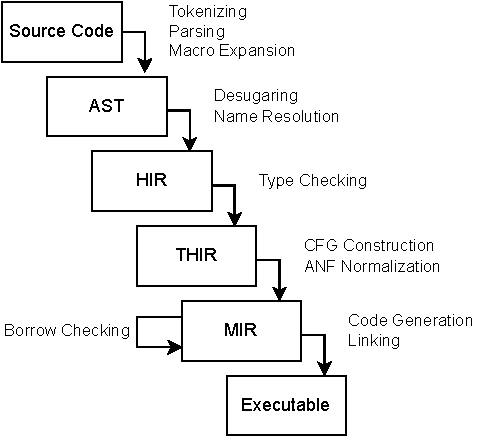
\includegraphics[width=0.7\linewidth]{./rustc-stages.pdf}
	\caption{Diagram providing an overview of the Rustc Compiler Stages}
	\label{fig:rust-stages}
\end{figure}

Figure \ref{fig:rust-stages} shows the the main compiler stages of Rustc and the associated data structure. The first data structure, that is extracted from the source code is the AST (short for abstract syntax tree), which is the result of parsing and expanding macros. 
Based on the AST, the high-level intermediate representation (short HIR) is created by resolving the names and desugaring some language constructs. The HIR contains accurate source labels, which map all nodes in the HIR to their source code locations. 
The HIR is then used as the basis for type checking returning the typed high-level intermediate representation (short THIR), which annotates every node with its type. THIR also lowers some additional constructs like automatic dereferencing and overloading and more. In contrast to the previous representations, "[t]he THIR only represents bodies, i.e. <<executable code>>; this includes function bodies [..]. Consequently, the THIR has no representation for items like \code{struct}s or \code{trait}s." \cite[p. 1]{noauthor_thir_nodate}
THIR will then be used to create the mid-level IR by drastically simplifying the language: The tree structure with complex expression of the THIR is turned in to a control-flow graph (short CFG) with basic blocks containing simple (i.e. non-nested) expressions.

Finally Rustc uses external tools \- like llvm \- to generate executable files and link them.



\chapter{Empirical Analysis of Use-Cases} \label{ch:analysis} 

Before designing a system for Rust, it makes sense to gain some understanding of how Rust is used. For this purpose we will look at two key features of Rust, that influence how an approachable verification should look like.
Firstly \code{unsafe} Rust, with a similar lack of guarantees to C, would make verification and specification significantly harder. But if the use of \code{unsafe} is limited, like intended by the language designers, it would allow us to focus on the save part of Rust and leave the verification of \code{unsafe} Rust to more complex verification systems, like Prusti \cite{astrauskas_leveraging_2019}.
Secondly with mutability being the main difference to the traditional domain of Refinement Types, estimating the need for covering this language feature is interesting. The prevalence of mutability should also inform the acceptable level of user effort.

Thus, the use-case analysis should answer the following questions about Rust code:
\begin{enumerate}
  \item How rare are uses of \code{unsafe}?
  \item How much effort is acceptable when specifying \code{unsafe} code?
  \item How common are mutable variables and references in Rust?
  \item How much effort is acceptable when specifying mutable variables and references in Rust?
\end{enumerate}

To check these assumptions an analysis of existing Rust code was performed\footnote{The source code is available at \url{https://gitlab.com/csicar/crates-analysis/}}. As a basis for the analysis, the Rust package registry \href{https://www.crates.io}{crates.io} was used. It contains the source code for both Rust libraries as well as various applications written in Rust (e.g. ripgrep). 

We analyzed all published Rust crates (Rust's version packages) on February 2nd 2022 on crates.io with at least 10 versions\footnote{The limit of 10 versions is used to eliminate inactive and placeholder packages}, which totals \numprint{11882} crates, containing \numprint{228263} files with a combined code-base size of over 64 million lines of Rust code (without comments and white space lines)\footnote{Calculated with \texttt{cloc}}. 

% from cloc
% ----------------------------------------------------------------------------------------
% Language                              files          blank        comment           code
% ----------------------------------------------------------------------------------------
% Rust                                 228263        5664979       10317162       64193670
% C                                     32945        1539542        1979846       13468919
% C++                                   18084        1263696        1093652        7956897
% JSON                                  15838           1897              0        6424252
% C/C++ Header                          31619        1152322        2015896        6284146
% XML                                    5142          25277          25773        4807556
% Assembly                               4146         534785         582345        2631991

The analysis parses these files and searches for certain AST patterns, which are subsequently extracted and saved.
Thanks to using the tree-sitter parsing framework, the analysis framework can easily be extended to other queries and languages.

\label{ss:unsafe-rust}\section{Unsafe Rust}

Firstly we will be answering the question of \code{unsafe} usage in Rust.
There is already some research on how \code{unsafe} is used in Rust. For example Astrauskas et al. \cite{astrauskas_how_2020} found, that about 76\% of crates did not use any unsafe. On top of that, unsafe signatures are only exposed by 34.7\% of crates, that use \code{unsafe}.

"The majority of crates (76.4\%) contain no unsafe features at all. Even in most crates that do contain unsafe blocks or functions, only a small fraction of the code is unsafe: for 92.3\% of all crates, the unsafe statement ratio is at most 10\%, i.e., up to 10\% of the codebase consists of unsafe blocks and unsafe functions." \cite[p. 13]{astrauskas_how_2020}
Our data seems to confirm this: \numprint{8044} of the \numprint{11882} crates (67.7\%) did not use any unsafe. 

Astrauskas et al. also found, that "however, with 21.3\% of crates containing some unsafe statements and – out of those crates – 24.6\% having an unsafe statement ratio of at least 20\%, we cannot claim that developers use unsafe Rust sparingly, i.e., they do not always follow the first principle of the Rust hypothesis." \cite[p. 14]{astrauskas_how_2020}

Although true, when analyzing unsafety for our use case, it makes sense to further distinguish between libraries and executables crates: Libraries are intended to be used by other Rust programs: Usage of unsafe in libraries may not be as problematic as in executables, because libraries are written once but used by many applications, justifying higher verification effort. 

In our analysis we found, that expectedly crates.io contains significantly more libraries than binaries\footnote{Libraries and Executables are distinguished by checking if they contain \code{bin} or \code{lib} target or one of the corresponding files according to the cargo naming convention.}: About \numprint{81.7}\% of crates contained just a library, \numprint{10.3}\% contained just an executable target and \numprint{10.3}\% contained both. 
We also found, that libraries are much more likely to use \code{unsafe} Rust.


\Cref{fig:unsafe-scatter} gives an overview over how \code{unsafe} sections are distributed in the crates.
\begin{figure}[h]
	\centering
	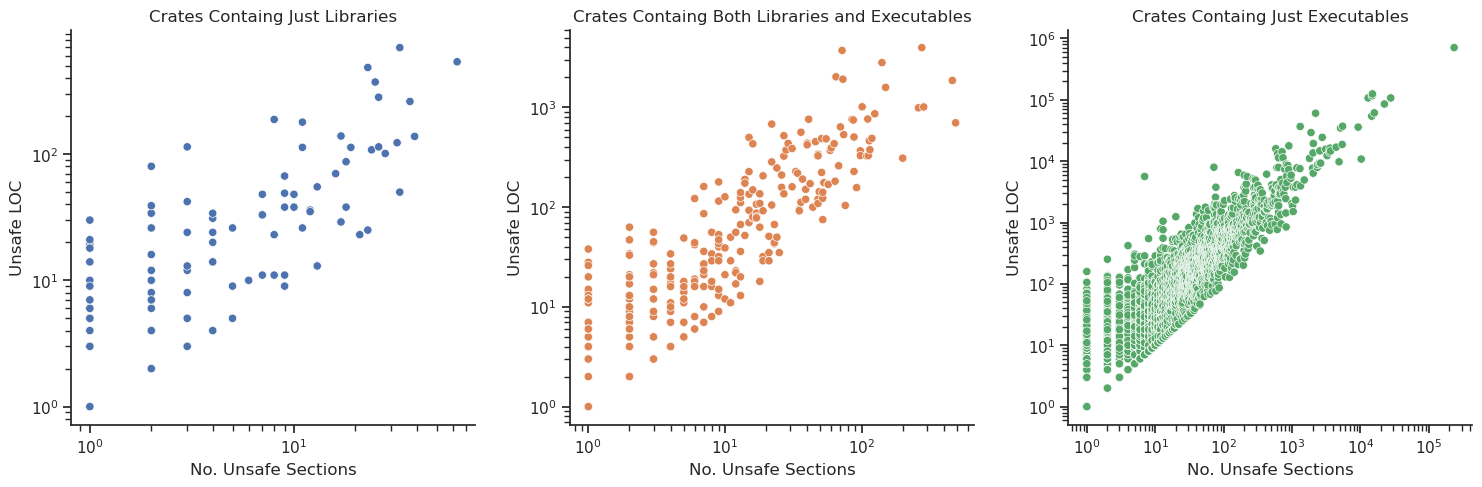
\includegraphics[width=0.99\linewidth, clip, trim={0.2cm 0.2cm 0.2cm 0.2cm}]{../scatter-occurences-vs-loc.png}
	\caption{Scatter plot of a point representing creates, relating the number of unsafe occurrences to the number of unsafe LOC}
	\label{fig:unsafe-scatter}
\end{figure}
\todo{Plots in Figure 3.1 sind ein bisschen klein
- Außerdem ist in Figure 3.1 vielleicht eher die durchschnittliche unsafe-Block-Größe interessant? Dann bräuchte die y-Achse keine Log-Skala}

\Cref{tab:unsafe-uses-by-crate} shows the result of our analysis: The total number of unsafe uses in an order of magnitude higher for binaries compared to libraries.
The data in the table includes all crates except the outlier \code{windows-0.32.0}, which alone contains \numprint{233608} uses of \code{unsafe}. Nearly $2 / 3$ of all other library uses of \code{unsafe} combined.
Looking at the distribution of unsafe uses in Figure \ref{fig:unsafe-ecdf}, we can see, that this is an exception: Most other libraries do not use that much unsafe statements. We can also see, that even if a executable crate uses \code{unsafe}, it uses few. Note the difference in x- and y-axis scaling: No executable contains more than 63 occurrences on \code{unsafe} blocks, but more than 10\% of libraries contain more than 63 \code{unsafe} sections.
On average, a library contains about 63 \code{unsafe} sections, while crates with binaries contain on average about 6 \code{unsafe} sections.


% \begin{figure}[h]
% 	\centering
% 	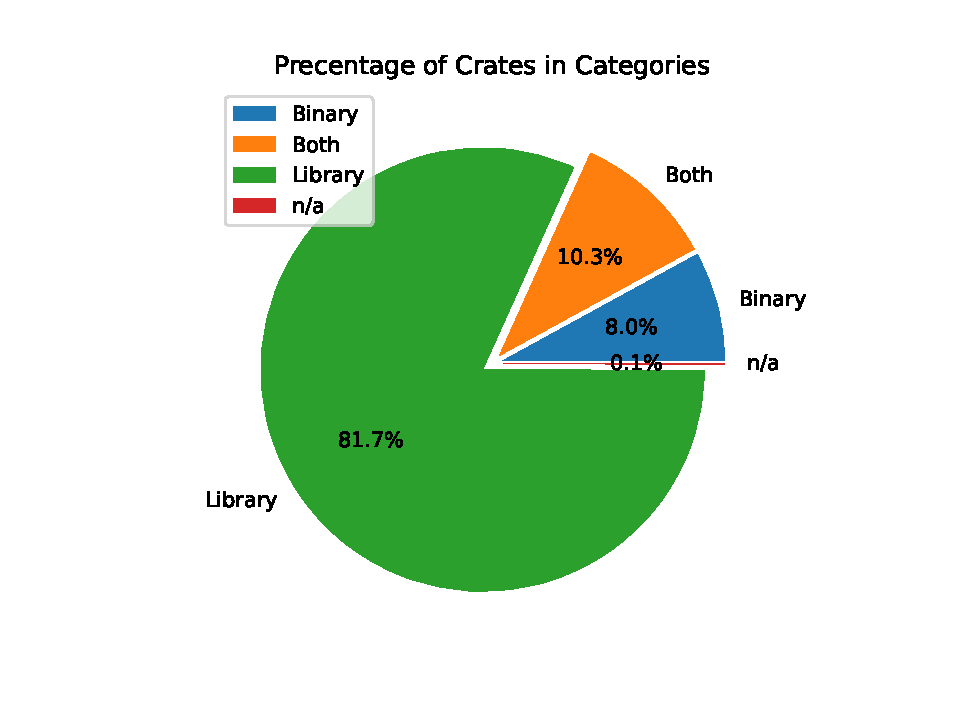
\includegraphics[width=0.5\linewidth, clip, trim={1cm 1cm 2cm 0.5cm}]{../crate_types.pdf}
% 	\caption{Percentage of Crates, that Contain Libraries, Executables or Both}
% 	\label{fig:crate_types}
% \end{figure}

\begin{table}[h]
\centering
\begin{tabular}{l | r | r | r}
  & No. Crates & Total No. of Unsafe Sections & Total Unsafe LOC \\
 Crate contains & & &  \\
 \hline
 Library & \numprint{9707} & \numprint{382997} & \numprint{2166213} \\
 Both & \numprint{1224} & \numprint{7720} & \numprint{51004} \\
 Binary & \numprint{951} & \numprint{940} & \numprint{5873} \\
 \end{tabular}
\caption{Number of Unsafe Uses by Crate Category}
\label{tab:unsafe-uses-by-crate}
\end{table}



\begin{figure}[h]
	\centering
	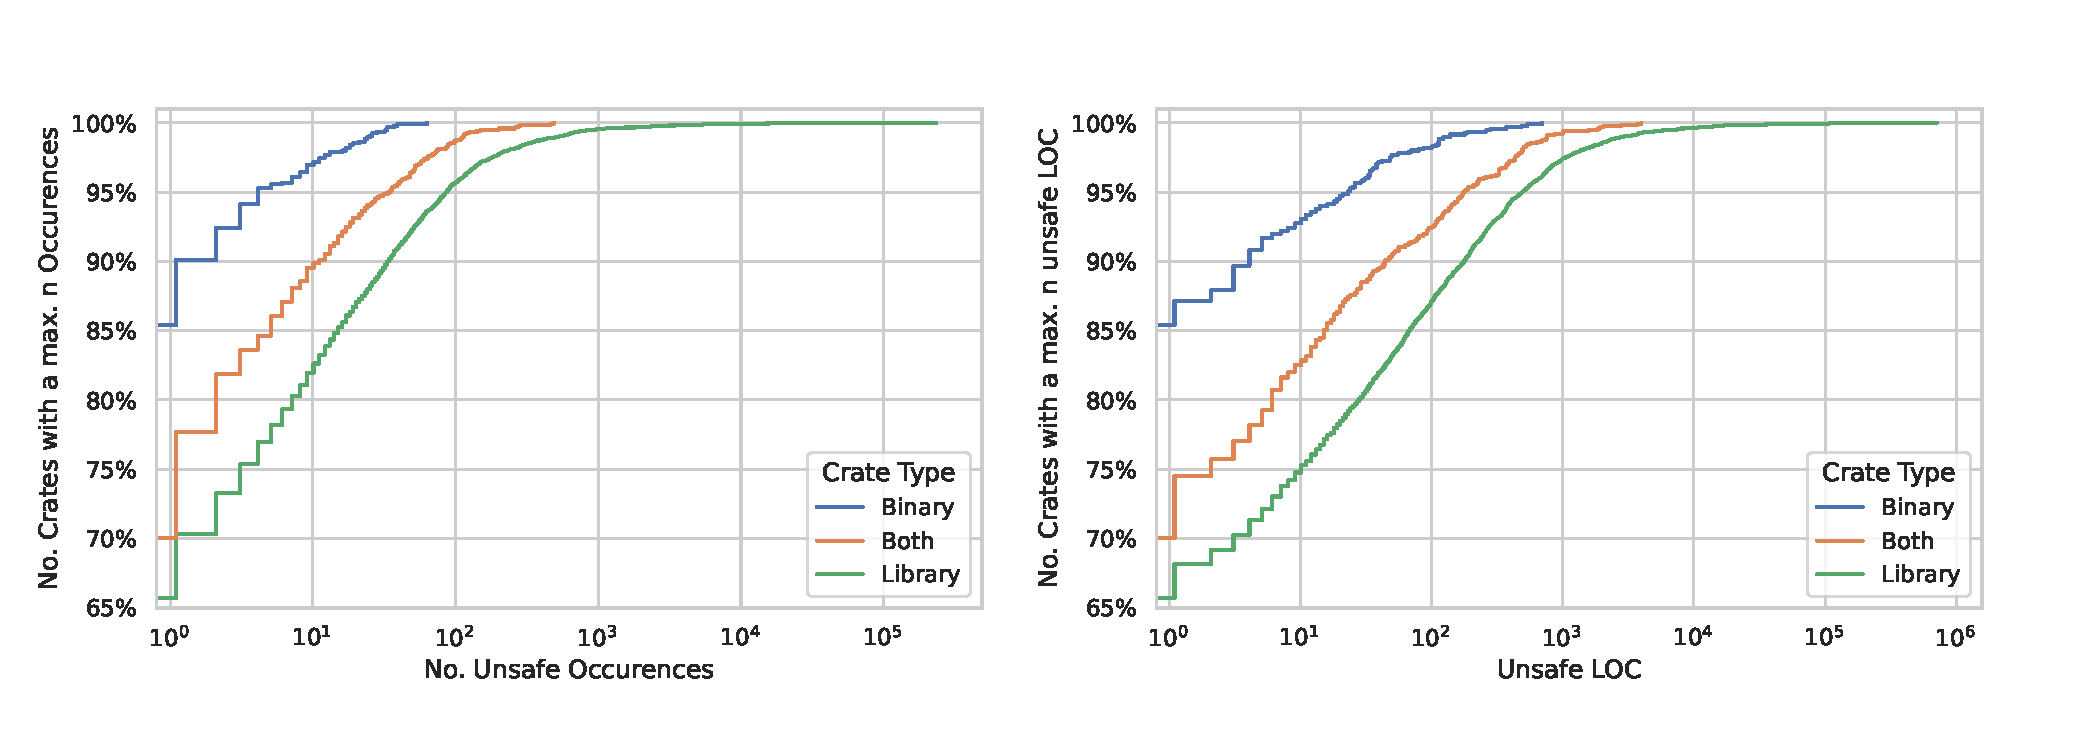
\includegraphics[width=0.99\linewidth, clip, trim={0.2cm 0.2cm 0.2cm 0.2cm}]{../ecdf-occurences-and-log-vs-no-crates.pdf}
	\caption{Cumulative, Logarithmic Histogram of the Amount of \code{unsafe} Uses in each Category}
	\label{fig:unsafe-ecdf}
\end{figure}



\label{sec:analysis-mutability} \section{Mutability}

Finally we will analyse how common mutable variables and references are used in Rust. 
The frequency of usage will inform the acceptable level of specification effort.

To analyse the dataset for usage patterns, we search the dataset for certain syntactical structures to infer mutability information about the following AST items:
\begin{itemize}
	\item \textbf{Local Variable Definitions} can be tracked with high confidence. They occur in function bodies and take the form: \code{let mut a = <expr>}
	\item \textbf{Parameters}, which are considered immutable if they are passed as immutable references or owned. They take the syntactic form: \code{mut a: i32} or \code{b: \&mut i32}
	\item \textbf{Function Definitions}, which are considered immutable, if all parameters considered immutable. They take the syntactic form: \code{fn f(mut a: i32, b: \&mut i32) \{ ... \}}
	\item \textbf{Arguments} are parts of a function call and can be arbitrary expression, which makes the tracking hard.
	\item \textbf{Function Calls}, which are considered immutable, if all arguments are considered immutable.
\end{itemize}

A total of around 52 million of these items were found in the dataset.

\Cref{fig:mutabillity_percentages} shows the ratio of mutable to immutable items. For each syntactical category, the percentages are relative to the total number of occurrences in the dataset.


\begin{figure}[h]
	\centering
	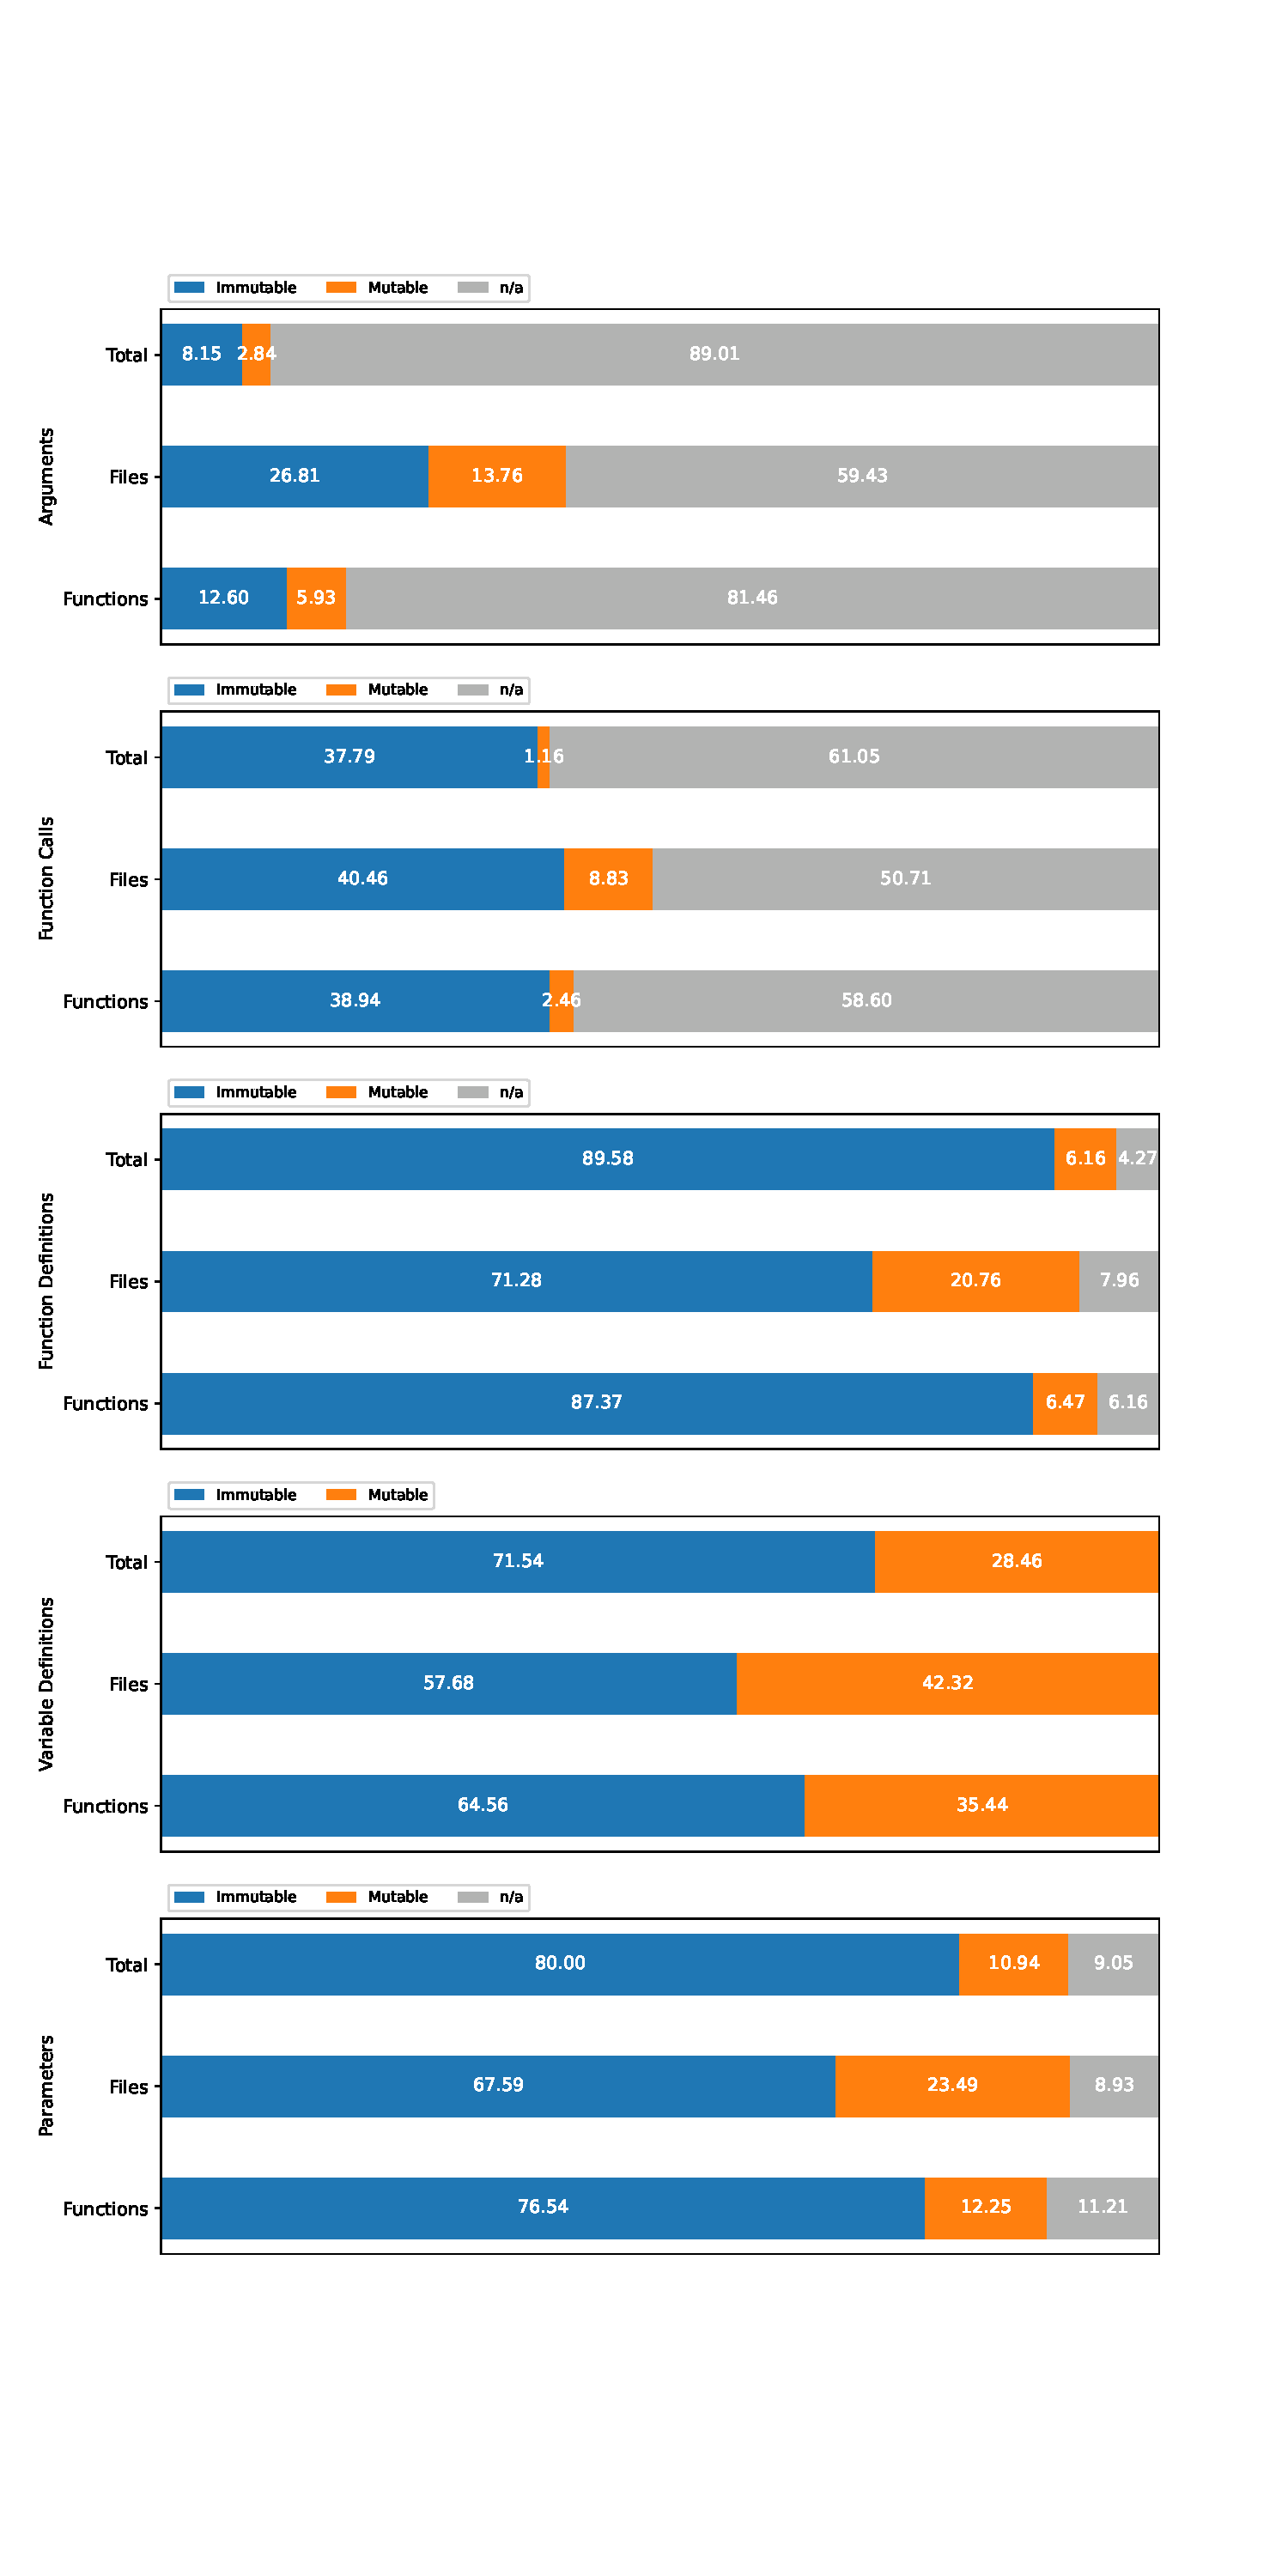
\includegraphics[width=0.9\linewidth, clip, trim={0.5cm 0.5cm 0.5cm 0.5cm}]{../mutability_by_category.pdf}
	\caption{Ratio of Immutable to Mutable Items of Different AST Nodes. Ratio is Relative to Total Number Of Occurrences}
	\label{fig:mutabillity_percentages}
\end{figure}

Unfortunately there are some areas, where the syntactic analysis is not sufficient. Namely the analysis of function calls and arguments, which is mainly caused by the uncertainty of mutability of complex arguments.
Luckily the data from function definitions and parameters can complete the picture: About 80\% of parameters are immutable and between about 10 and 20\% of parameters are mutable. And less than 10\% of functions have mutable parameters at all.
When it comes to local variables, Rust users are more liberal in their use of mutability:
About 30\% of local variables are defined mutable.

For verification this means, that the use of mutability is wide spread. Especially local variables are often mutable and should therefore a verification system should try to minimize the effort for the user. Mutable parameters are less common, but still need to be accounted for in verification.

\section{Conclusions}

For this thesis the following conclusion can be drawn:

\begin{itemize}
  \item Even though uses of \code{unsafe} are not rare, it is acceptable to ignore in favour of a simpler type system.
  \item Mutable variables are used very often and should therefore have very little associated specification effort.
  \item Mutable parameters are used less frequently justifying a higher specification effort, but their specification must still be possible.
\end{itemize}
\fi

\chapter{The MiniCorten Language} \label{ch:language} 

Rust's main disadvantage as a target language it its size: There is a lot of syntax and semantics that would need to be accounted. A lot of it even incidental to the verification. To reduce the complexity and amount of work, that needs to be done, we will focus on a subset of Rust described in this section.

The goal is to remove as much incidental complexity as possible without compromising to the central topic of research: How to extend LiquidTypes to mutability under the presence of Rust's ownership model.


\section{Syntax}

This subsection will introduce the syntax of MiniCorten, a language modelled after a simplified version of Rust, with the addition of refinement types.
To simplify the formal definitions and proofs, the language is restricted to A-Normal Form (short ANF), meaning arguments of expressions must be variables. ANF was described by \cite{sabry_reasoning_1993}. Note that the implementation does not have this restriction.

There are two namespaces for identifiers: $x \in \text{PVar}$ for variables of program variables and $\alpha \in \text{LVar}$ for variable in the refinement predicates. The syntax is defined by the following BNF-Grammar:

\begin{bnfgrammar}
  $program$  ::=
    $func\_decl$ * : function declarations
  ;;
  func\_decl ::=
    $ident$( $param$ * ) -> $\tau$ \{ $s$ \}
  ;;
  $param$ ::= $x$ \ccolon  $\tau$
  ;;
  $s$: stmt 
  ::=
    $e$                                                   : expression
    | $s_1$; $s_2$                                        : sequence
    | let mut? $x$ = $e$                                  : declaration
    | $x$ = $e$                                           : assignment
    | let $x_v$ = $x_f$($x_1, \dots, x_n$)                : function call
    | while ($x$) \{ $s$ \}                               : while loop
    | if $e_c$ \{ $s_t$ \} else \{ $s_e$ \}               : if statement
    | relax\_ctx!\{ $\varphi$* ; ($x$ \ccolon $\tau$)* \} : context relaxation
  ;;
  $e$                                              : expression 
  ::=
    $x$                                         : variable reference
    | $lit$                                         : constant
    | $e \odot e$                                   : binary operation
    | * $x$                                     : dereference
    | \& $x$                                    : immutable reference
    | \&mut $x$                                 : mutable reference
    | $e$ as $\tau$                                : type relaxation
  ;;
  $\tau$ : type ::= ty!\{ $\alpha$ \ccolon $b$ \cmid $\varphi$ \} : refinement type
  ;;
  $\varphi$ : pred ::=
    $ref\_pred$                                     : predicate for a reference type
    | $value\_pred$                                 : predicate for a value type
  ;;
  $ref\_pred$ ::=
    $logic\_ident$ = \& $ident$
    | $ref\_pred$ \cdisj $ref\_pred$         : mutable reference
  ;;
  $value\_pred$ ::=
    $\alpha$                                 : variable
  | $v$                                      : literal
  | $value\_pred \odot value\_pred$          : binary op
  | ! $value\_pred$                          : negation
  ;;
  $b$: base\_ty ::=
    i32                     : integer
    | unit                  : unit type
    | bool                  : boolean
    | \& $b$                : immutable reference
    | \&mut $b$             : mutable reference
  ;;
  $v$: lit ::=
      0,1,...,n             : integer
    | true                  : boolean true
    | false                 : boolean false
    | ()                    : unit value
  ;;
  $\odot$: bin\_op ::= $\wedge$ | $\vee$ | $\geq$ | $+$ | $=$
\end{bnfgrammar}

Most constructs are standard, the main difference being the addition of refinement types, that consist of a logic variable $\alpha$, a base type $b$ (from the target language) and a predicate $\varphi$. Intuitively this means, that the value inhabiting that type satisfied the $\varphi$ in $\alpha$ represents the value. 

\section{Semantics}

The semantics are mostly standard. The main difference being that Rust and our simplified language enable most statements to be used in place of an expression. The value is determined by the last statement in the sequence. For example If-Expressions, sequences of statements and function all follow this rule: Their (return) value is determined by the last statement or expression in the sequence.

The semantics loosely based on Jung's MiniRust \cite{jung_minirust_2022}.

Another difference between Rust and MiniCorten is of course the addition of refinement types.

In terms of the formal description, the rules are similar to Pierce's \cite[p. 166f]{pierce_types_2002-3} "Reference" language. % Also: Semantik von programmiersprachen WhileT p.45
The main difference is, that in Rust, every piece of data has a unique, known owner. This fact makes the concept of locations redundant. Instead we treat $\code{ref}(x)$ as a value itself. The following definitions show the new execution rules.

\begin{definition}[Execution-State]
  The execution state is a partial function from program variables to values: $\sigma : \text{PVar} \rightharpoonup \text{Value}$. 
\end{definition}


\begin{definition}[Evaluation of Expressions: $\bbracket{e} \sigma$ ]
  \begin{align*}
   \bbracket{v} \sigma &= v \\
   \bbracket{x} \sigma &= \sigma(x) \\
   \bbracket{e_1 + e_2} \sigma &= \bbracket{e_1} \sigma + \bbracket{e_2} \sigma \\
   \bbracket{*x} \sigma &= \sigma(y) \qquad \text{if } \sigma(x) = \code{ref}(y) \\
   \bbracket{\code{\&mut } x} \sigma &= \code{ref}(x) \\
   \bbracket{e \code{ as } \tau} \sigma &= \bbracket{e}\sigma \\
  \end{align*}
 \end{definition}
 

\begin{definition}[Declaration Environment]
  The environment of function declarations is constant and globally known. It is defined as a partial function $\Sigma : \text{Fn-Name} \rightharpoonup (n, s)$ where $n$ is the number of arguments and $s$ is the body of the function
\end{definition}

\begin{definition}[Small-Step Semantics of MiniCorten: $\tuple{e}{\sigma} \leadsto \tuple{e'}{\sigma'}$]

$$\begin{gathered}
  \inferrule*[left=SS-Assign\rulelabel{SS-Assign}]
    {\star}
    {\tuple{x = e }{ \sigma } \leadsto \tuple{\code{unit} }{ \sigma[x \mapsto \bbracket{e}\sigma]}}
  \\
  \inferrule*[left=SS-Assign-Ref\rulelabel{SS-Assign-Ref}]
    {\sigma(x) = \&y}
    {\tuple{*x = e }{ \sigma } \leadsto \tuple{\code{unit} }{ \sigma[y \mapsto \bbracket{e}\sigma]}}
  \\
  \inferrule*[left=SS-Decl\rulelabel{SS-Decl}]
    {\star}
    {\tuple{\code{let } x = e}{\sigma} \leadsto \tuple{unit}{\sigma[ x \mapsto \bbracket{e}\sigma]}}
  \\
  \inferrule*[left=SS-Seq-Inner\rulelabel{SS-Seq-Inner}]
      {\tuple{e_1 }{ \sigma } \leadsto \tuple{e_1' }{ \sigma'}}
      {\tuple{e_1; e_2 }{ \sigma } \leadsto \tuple{e_1'; e_2 }{ \sigma'}}
  \inferrule*[left=SS-Seq-N\rulelabel{SS-Seq-N}]
    {\star}
    {\tuple{\code{unit}; e_2 }{ \sigma } \leadsto \tuple{e_2 }{ \sigma'}}
  \\
  \inferrule*[left=SS-IF-T\rulelabel{SS-IF-T}]
    {\bbracket{x} \sigma = \code{true}}
    {\tuple{\code{if } x\ \{ s_t \} \code { else } \{ s_e \} }{\sigma} \leadsto \tuple{s_t}{\sigma}}
  \inferrule*[left=SS-IF-F\rulelabel{SS-IF-F}]
    {\bbracket{x}\sigma = \code{false}}
    {\tuple{\code{if } x\ \{ s_t \} \code { else } \{ s_e \} }{\sigma} \leadsto \tuple{s_e}{\sigma}}
  \\
  \inferrule*[left=SS-While\rulelabel{SS-While}]
    {\star}
    {
      \tuple{ \code{while } e_c\ \{\ s_b \}}{\sigma}
      \leadsto
      \tuple{ \code{if } e_c \{ s_b;  \code{while } e_c \{ s_b \} \} { \code{ else } } \{ \code{unit} \} }{\sigma}
    }
  \\
  \inferrule*[left=SS-Relax\rulelabel{SS-Relax}]
    {\star}
    {\tuple{\code{relax\_ctx!\{ ... \}}}{\sigma} \leadsto \tuple{\code{unit}}{\sigma}}
  \\
  \inferrule*[left=SS-Call\rulelabel{SS-Call}]
    {\tuple{\Sigma(f)[arg_1 \triangleright x_1, \dots, arg_n \triangleright x_n]}{\sigma} \leadsto \tuple{v_r}{\sigma'} }
    {\tuple{f(x_1, \dots, x_2)}{\sigma} \leadsto \tuple{v_r}{\sigma' \oplus \sigma}}
\end{gathered}$$

where $$(\sigma' \oplus \sigma)(x) =
  \begin{cases}
    \sigma(x) & \text{if } x = arg_i \\
    \sigma'(x) & \text{if } x \in \dom(\sigma) \cap \dom(\sigma')\\
    \sigma(x) & \text{otherwise }
  \end{cases}$$
\end{definition}


The \cref{rule:SS-Call} rule does not scope the variables from the callee to the caller. This is actually fine, because by definition variable names are distinct. Therefore only the arguments need to be replaced in the resulting state.

\chapter{The Refinement Type System} \label{ch:type-system}


\section{Features}

This subsection will explain some of the key features of the Corten type system.
Corten is directly embedded in Rust using two macros. Firstly the macro \code{ty!} can be used in place of a Rust type and adds a predicate to the Rust type, that any inhabitant of that type must satisfy. For example, the type \code{ty!\{ v : i32 | v >= 0\}} stipulates, that a value of Rust type \code{i32} is positive. The second macro is \code{relax\_ctx!\{ ... \}} which will be explained in subsection \ref{subsec:atomic-updates}.

\subsection{Decidable, Conservative Subtyping}

Having a decidable subtyping system is essential to making it feasible in practice: A developer expects type checking to be automatic and part of compilation without additional effort. There is no need for user interaction, if the SMT solver can automatically verify the program.

\subsection{Mutable Values}

As seen in \cref{sec:analysis-mutability}, mutable declarations are quite common in Rust. Therefore handling them is essential for Corten.
To explain the problems that mutable values can cause, consider the problem seen in \cref{list:mutable-values}: Suppose the value given to \code{i} is known to be positive, which is expressed by the type $\{ v_1 : i32 \mid v_1 > 0\}$, then assigning a new value to \code{i} may change the type. Notably, the new value's type might depend on the old value, which is the case here: \code{i + 1} has type $\{ v_2 : i32 \mid v_2 = v_1 - 1\}$.
Corten elected to treat predicates as immutable, meaning assigning to a variable will not change the old predicates, that was associated with the variable.
Therefore assigning a new value to a variable will give that variable a new type, but \- crucially \- keep the logic variable in the typing context, which means that types of other variables can still refer to it. Logic variables, that are no longer associated with a program variable (like $v_1$), are called unassociated variables.
That means, that the number of predicates in the context increases with every new value assignment.
In the example, the typing context initially contains the predicate $v_1 > 0$ and the association of $\{i \mapsto v_1\}$. After the assignment, the predicate $v_2 = v_1 + 1$ is \textit{added} to the context and the association is \textit{changed} to $\{i \mapsto v_2\}$
% In the example, the typing context at the end of the function body contains $v_1$, $v_2$ and their predicates and the association of \code{i} to $v_2$.

There are other approaches for handling changing values in refinement types, which will be described and compared in \ref{subsec:related-work-mutability}.


\begin{listing}[ht]
  \begin{minted}[fontsize=\footnotesize, texcomments]{rust}
    fn decr() -> ty!{ v: i32 | v >= 0 } {
        let mut i = ...;    // i : $\{ v_1 : i32 \mid v_1 > 0 \}$
        i = i - 1;          // i : $\{ v_2 : i32 \mid v_2 == v_1 - 1 \}$
        i
    }
  \end{minted}
  \caption{Example demonstrating why predicates and mutable values may cause problems}
  \label{lst:mutable-values}
\end{listing}

\label{subsec:mutable-references}\subsection{Mutable References}

Besides the mutation of values, mutable references are also common in Rust, which is underpinned by the analysis, which found more than 10\% of parameters to be mutable.
% The key difference to Refinement Type Systems for functional languages to Rust it the pervasive use of mutation. Therefore the most important feature of Corten it the support for mutation and also mutable references.

Corten has two ways of dealing with assignment to mutable references: If the reference destination is known, the destination's type will be updated with the assigned values type (i.e. strong update). If there are multiple possible reference destinations, Corten will require the assigned value to satisfy the predicates of all possible destinations (i.e. weak updates). This is a standard approach (e.g. \cite{kloos_asynchronous_2015}), but more precise in Rust: The set of possible destinations only grows, when it depends on the execution of an optional control flow path. This means most of the time, strong updates are possible and weak updates are only needed if the reference destination is actually dynamic (i.e. dependent on the execution) \footnote{It would also be possible to encode the path condition in the reference type, but this was decided against for the stated goal of simplicity for the user}

The problem with mutable references is possibility of aliasing. Aliasing is problematic, because it might create interdependencies between the types of different variables: If one variable is changed, it might affect wether another variable is typed correctly. In \cref{lst:mutation-strong} the return value \code{a} is affected by changes done to a different variable \code{a}. Conservative approximation requires, that all possible effects must be tracked.

The key idea is, that reference types constrains the reference target, while the value owner's type constrains the value.
Because of the ownership system, Corten can accurately track references, which are phrased as predicates.
In the example, \code{b = \&mut a} and \code{\&mut a} will have inferred type \code{\{ r : \&mut | r == \& a \}}, meaning any inhabitant of this type can at most refer to the variable called \code{y}.
When a new value is assigned to \code{*b}, the type system will look at the typing context to find out what \code{b} might refer to. In this case \code{a} is the \textit{only} possible target und we can therefore \textit{update} its type. I.e. in type system, \code{*b = 0} will change the type of \code{a} to \code{\{ s : i32 | s == 0 \}}, but the type of \code{b} stays the same (because it still refers to the same location). We call this kind of assignment a strong assignment, as it can change the type. 

This is sensible, because in Rust's ownership system, \code{a} must be the unique owner of the memory belonging to \code{a}, meaning no other value predicate can be affected by the change.

\begin{listing}[ht]
  \begin{minted}[fontsize=\footnotesize, texcomments]{rust}
    fn client() -> ty!{ v: i32 | v == 4 } {
        let a = 2;       // a : $\{ v_1 : i32 \mid v_1 == 2 \}$
        let b = &mut a;  // b : $\{ v_2 : &i32 \mid v_2 == &a \}$
        *b = 0; // changes a's value and type
        let c = &mut b;  // c : $\{ v_3 : &i32 \mid v_3 == &b \}$
        **c = 4; // changes a's value and type
        a
    }
  \end{minted}
  \caption{Example demonstrating interdependencies between mutable references}
  \label{lst:mutation-strong}
\end{listing}

Note, that the type can only be changed because we know exactly what \code{b} refers to. If there is ambiguity about the destination of a reference, strong updates are no longer possible.

To support these use cases, Corten also supports weak updates, which can not change types, but allow assigning to ambiguous reference destinations.
\Cref{lst:mutation-weak} demonstrates how ambiguity about the reference destination may emerge: Depending on the if condition, \code{res} could refer to either \code{y} or \code{z}.
Naturally, we can weaken the reference type to \code{ty!\{ r1 : \&mut i32 | r1 == \&y || r1 == \&z \}}, meaning \code{res} could refer to either \code{y} or \code{z}.
Because the destination is ambiguous, assigning to \code{*res} can not change the type of \code{y} or \code{z}, which is the case if the type of the assigned value is at least as specific as the types of all possible reference destinations.

\begin{listing}[ht]
  \begin{minted}[fontsize=\footnotesize, texcomments]{rust}
    fn weak_updates(x : ty!{ x1 : i32 }) -> ty!{ v : i32 | v > 2 * x1 + 10 } {
      let mut y = x as ty!{ y1 : i32 | y1 >= x1 };
      let mut z = x + 10 as ty!{ z1 : i32 | z1 >= x1 + 10 };
      let mut res;
      if x > 0 {
        res = &mut y as ty!{ r : &mut | r == &y || r == &z };
                      // branches of if need same type => weaken
      } else {
        res = &mut z as ty!{ r : &mut | r == &y || r == &z };
      }
      *res = x + 11; // res could refer to b or c 
                    // -> assigned value must satisfy both types
      y + z
    }
  \end{minted}
  \caption{Example demonstrating weak updates}
  \label{lst:mutation-weak}
\end{listing}

An intricacy about conservative reference tracking are functions, that return references. In Rust this is possible, if the reference was passed as an argument: The function signature \code{fn f(a : \&mut T, b : \&mut T) -> \&mut T} would allow \code{f} to return either a reference to \code{a} or \code{b}. For the callee knowing where the returned value points to, is important because the type of dereferencing it depends on that knowledge. Consequently, for the return type to be conservative, it must state every possible reference destination.


\label{subsec:path-sensitivify}\subsection{Path Sensitivity}

Firstly, the type system is path sensitive, meaning that the type system is aware of necessary XXX that need to be passed for an expression to be evaluated. For example listing \ref{lst:max-path-sensitive} shows a function computing the maximum of its inputs. In the then branch, $a$ is only a maximum of $a$ and $b$, because the condition $a > b$ implies it. Corten will symbolically evaluate the condition and store it in its typing context.

\begin{listing}[ht]
  \begin{minted}[fontsize=\footnotesize]{rust}
    fn max(a : ty!{ av: i32 }, b: ty!{ bv: i32 })
        -> ty!{ v: i32 | v >= av && v >= bv} {
        if a > b {
          a as ty!{ x : i32 | x >= av && x >= bv }
        } else {
          b
        }
    }
  \end{minted}
  \caption{Function computing the maximum of its inputs; guaranteeing that the returned value is larger than its inputs}
  \label{lst:max-path-sensitive}
\end{listing}


- inference
- also with mutations


\label{subsec:strong-type-updates}\subsection{Strong Type Updates}

\begin{listing}[ht]
  \begin{minted}[fontsize=\footnotesize]{rust}
    fn strong_updates(b: ty!{ bv: i32 | bv > 0}) -> ty!{ v: i32 | v > 2} {
        let mut a = 2;
        a = a + b;
        a
    }
  \end{minted}
  \caption{Example of changes to \code{a}'s value affecting its type}
  \label{lst:strong-updates}
\end{listing}



\label{sec:modularity}\subsection{Modularity}

For a verification system to be scalable, it needs to be able modularize a proof. Corten can propagate type information across function calls and by taking advantage of Rust's ownership system, it can do so very accurately. Listing \ref{lst:modular-calls} shows, how an incrementing function \code{inc} can be specified: \code{inc} signature stipulates, that it can be called with any \code{i32} (given the name \code{a1}) and will return a value \code{a2}, which equals \code{a1 + 1}. Only the signature of \code{inc} is necessary for the type checking of \code{client}. 

Notice, that all of the type information about \code{y} is preserved when \code{inc(x)} is called. There are no further annotations needed to type check this program. This is possible, because in safe Rust, any (externally observable) mutation done by a function must be part of the function signature. Corten expands on this, by enabling the user specify exactly how a referenced value is mutated.

\begin{listing}[ht]
  \begin{minted}[fontsize=\footnotesize]{rust}
    fn inc(a: &mut ty!{ a1: i32 => a2 | a2 == a1 + 1 }) {
      *a = *a + 1;
    }
    fn client(mut x: ty!{ xv: i32 | xv > 2 }) -> ty!{ v: i32 | v > 7 } {
      let mut y = 2;
      inc(&mut x); inc(&mut x);
      inc(&mut y)
      x + y
    }
  \end{minted}
  \caption{Example showing how Corten allows for accurate type checking in the presence of function calls }
  \label{lst:modular-calls}
\end{listing}




\label{subsec:atomic-updates}\subsection{Atomic Updates}

Complex mutation patterns can result in complex interdependencies. We deem it necessary to allow different types to refer to each other. 
The properties of arguments might depend on each other, consequently their refinement types should be able to refer to each other.

The listing \ref{lst:mutual-reference} is extract from the evaluation example \ref{subsec:evaluation-gauss}. It requires establishing an invariant, where \code{i} has the predicate $\geq 0$ and \code{sum} has the predicate $= i \cdot n$.

Attempting to update one type at a time, will not yield the desired result. If \code{i} is updated first, then it is not possible to establish \code{sum}'s type, because \code{i}'s type is no longer expressive enough.
If \code{sum} is updated first, we can establish its type, but once \code{i} is updated, it will refer to a different logic variable for \code{i} than \code{sum}. If we tried to carry the information, that the two logic variables are the same in the type, it would no longer be an invariant, because reassigning the value would invalidate it\footnote{
  For this use-case, it might also be possible to relax a single variable at a time, by renaming the logic variables to their old names after the subtyping relation is shown. This approach was not chosen, because its influence on correctness are hard to assess.
}.

\begin{listing}[ht]
  \begin{minted}[fontsize=\footnotesize, autogobble]{rust}
    let sum = 0;
    let i = 0;
    
    relax_ctx!{
      i: ty!{ iv : i32 | iv > 0  },
      sum: ty!{ sv: i32 | 2 * sv == iv * (iv + 1) }
    }

    i = i + 1;
    sum = sun + i;

  \end{minted}
  \caption{Demonstration of interdependent types}
  \label{lst:mutual-reference}
\end{listing}

For this purpose, Corten provides a mechanism for the programmer to instruct Corten to relax all variables at once \- named \code{relax\_ctx}. The syntax is similar to the refinement type syntax, but allows for multiple variables to be described at a time. The type system will check all refinement types at once, resulting in the successful type checking of the example.

\section{Type System}

The following sections will introduce the type checking rules of Corten. We assume the program has passed the Rust type checking rules, meaning (non-refined) type- and ownership-checking was successful.

\begin{definition}[Typing Context $\Gamma = (\mu, \Phi)$]
  The typing context, consisting of an injective function $\mu : \text{PVar} \rightharpoonup \text{LVar}$, that is used for tracking the current logic variable associated with a program variables and a set of predicates $\Phi$, which constrains the logic variables in the image of $\mu$, holds the relevant dynamic state for the various type checking rules.
  $\mu$ must contain a logic variable for every program variable and $\Phi$ can contain additional logic variables not found in the image of $\mu$.

  We abbreviate $(\mu, \Phi \wedge \varphi)$ to $\Gamma, \varphi$ for the addition of $\varphi$ to the constraint set, $(\mu[x \mapsto \alpha], \Phi)$ to $\Gamma[x \mapsto \alpha]$ for the update of the mapping for program variable $x$ to $\alpha$ and 
  $\mu(x)$ to $\Gamma(x)$ for accessing to the logic variable associated with $x$.
\end{definition}

We start with the rule for checking function declarations.
Without loss of generality, we assume arguments are ordered by their type: First immutable / owned arguments and then mutable arguments.

\begin{definition}[Function Declaration Type Checking]
When handling mutable references in parameters some subtleties need to be considered. The function can change both the referenced \textit{value} as well as the reference \textit{location}. To describe the referenced value is normally done using the $\{ \alpha \mid \alpha \doteq \&b\}$ syntax. The question arises: If $\alpha$ was the logic variable for a parameter, what should be the analog for $b$? In contrast to local variables, there is no variable representing the referenced value for parameters. As seen in section \ref{subsec:mutable-references}, using the dereference operator would come with a lot of complications.
Instead we introduce $arg^i_n$, a special variable denoting the initial abstract value (i.e. stack location), that the mutable reference of argument $n$ points to. $i$ denotes the level of nesting: For the $n$th parameter with the Rust type \code{\&mut \&mut i32} we would generate $arg^1_n$ and $arg^2_n$.

\begin{gather*}
  \inferrule*[left=Fn-Decl]
    { (\{ a_1 \mapsto \alpha_1, b_1 \mapsto \delta_1 \}, \varphi^\alpha_1 \wedge \dots \wedge \delta_1 = arg^1_1 \wedge \varphi^\beta_1 \wedge \dots ) \vdash \bar s \Rightarrow \Gamma'
      \\ \Gamma' \vdash s_{res} : \tau_{res} \Rightarrow \Gamma''
      \\ \Gamma'' \vdash \tau_{res} \preceq \tau
      \\ \Gamma'' \preceq (\{\beta_1 \mapsto \gamma_1\}, \varphi^\gamma_1 )
    }
    {\code{fn } f(a_1 : \{ \alpha_1 \mid \varphi^\alpha_1 \}, \dots, b_1 : \{ \beta_1 \mid \varphi^\beta_1 \Rightarrow \gamma_1 \mid \varphi^\gamma_1\}) \to \tau \{ \bar s; s_{res} \}}
\end{gather*}
\end{definition}

Next, we introduce the Rule for checking the subtype relation.
\begin{definition}[Sub-Typing Rule: $\Gamma \vdash \tau \preceq \tau'$]
A type $\tau$ is a subtype of $\tau'$ in the context $\Gamma$, if the predicate of the supertype imply the predicate of the subtype. Corten uses a decidable, propositional logic with the theories of equality and linear arithmetic. 
Before dispatching a request to the SMT solver, the supertype's logic variable is substituted for the subtype's variable to the predicate to refer to the same variable.

\[
  \inferrule*[left=$\preceq$-Ty]
    {\text{SMT-Valid}(\Phi \wedge \varphi'[\beta \triangleright \alpha ] \implies \varphi)}
    {\Gamma = (\mu, \Phi) \vdash \{ \alpha \mid \varphi\} \preceq \{ \beta \mid \varphi' \}}
\]
\end{definition}
% alternative (should be equivalent):

% \[
%   \inferrule*[left=$\preceq$-Ty-Alt]
%     {
%       \Gamma[f \mapsto \alpha], \varphi \preceq \Gamma[f \mapsto \beta], \varphi'
%       \\ f \text{ fresh}
%     }
%     {\Gamma \vdash \{ \alpha \mid \varphi\} \preceq \{ \beta \mid \varphi' \}}
% \]

Note that, $\Gamma \vdash \tau \preceq \tau'$ can be rephrased in terms of $\Gamma \preceq \Gamma'$ by introducing a fresh variable with the predicates $\tau$ and $\tau'$. The rephrased form is equivalent, but rephrasing the sub context rule in terms of sub-typing is in general not possible: Because all constraints need to be satisfied at the same time when checking for sub-contexts, just checking each variable at a time would be a weaker proposition.

\begin{definition}[Sub-Context Rules: $\Gamma \preceq \Gamma'$]

In contrast to other refinement type systems, Corten allows types in the context to refer to one another.
For example a type specifications \code{a : \{ $\alpha$ : i32 | $\alpha$ > $\beta$\}, b:  \{ $\beta$: i32 | $\beta$ != $\alpha$\}} would be valid and result in the context $\Gamma = (\emptyset, \alpha \neq \beta \wedge \beta \geq \alpha)$. In the example, the value $0$ i a valid inhabitant of \code{a}'s type as long as $\code{b} \geq 1$.

The rule \textsc{$\preceq$-Ctx} serves the purpose of allowing these interdependencies between predicates while still providing an applicable concept of subtyping: As long as the set of predicates in $\Gamma'$ imply the predicates for $\Gamma$, the sub-context relation is satisfied and $\Gamma'$ and $\Gamma$ is called the super-context and sub-context respectively. 
To be more precise: The rule needs to relate the predicates for each \textit{program} variable with the opposing predicates for that program variable. The substitution $\Phi'[\mu'(x) \triangleright \mu(x)\ \mid x \in \dom(\mu)]$ forces the logic variable associated with \code{x} in $\Gamma'$ to be substituted by the logic variable $\mu(x)$ , which is associated with \code{x} in $\Gamma'$.

The domain restriction ensures, that the sub-context does not contain additional program variables, which would leave unconstrained variables in the antecedent

\[
  \inferrule*[left=$\preceq$-Ctx]
    {
      \text{SMT-Valid}(\Phi'[\mu'(x) \triangleright \mu(x)\ \mid x \in \dom(\mu')] \implies \Phi)
      \\ \dom(\mu') \subseteq \dom(\mu)
    }
    {(\mu, \Phi) \preceq (\mu', \Phi')}
\]
\end{definition}


\begin{definition}[Fresh Variable $\Gamma \vdash \alpha \text{ fresh}$]

Corten requires that new logic variables are distinct from all others. The rule ensures that $\alpha$ is a free variable in $\Gamma = (\mu, \Phi)$:
  $$\Gamma \vdash \alpha \text{ fresh} \text{ iff } \alpha \notin FV(\Phi) \cup \img(\mu)$$
\end{definition}

\begin{definition}[Expression Constraint $\alpha \simeq \bbracket{e}\Gamma$]
An expression constraint is used to restrict $\alpha$ to (as close to) the value of expression $e$. For instance, typing the expression \code{b + 3} should get the strongest type $\alpha \doteq \beta + 3$ where $\beta$ is the logic variable for \code{b}.
It could also be possible that an expression can not be directly translated, like operations not allowed by the logic. In that case, the expression will be conservatively approximated by the predicate \code{true}.

\begin{align*}
  \alpha \simeq \bbracket{v}\Gamma &= \alpha \doteq v
  \\ \alpha \simeq \bbracket{x_1 \odot x_2}\Gamma &= \alpha \doteq (x_1 \odot x_2) &&\text{if }\odot\text{ allowed}
  \\ \alpha \simeq \bbracket{x}\Gamma &= \alpha \doteq \mu(x)
  \\ \alpha \simeq \bbracket{\&y}\Gamma &= \alpha \doteq \&y
  \\ \alpha \simeq \bbracket{e}\Gamma &= \text{true} &&\text{otherwise}
\end{align*}
\end{definition}

\begin{definition}[Expressions Typing: $\Gamma \vdash e : \tau$]


$$ \begin{gathered}
  \inferrule*[left=Lit\rulelabel{Lit}]
    {\alpha \text{ fresh}}
    {\Gamma \vdash v: \{ \alpha : b \mid \alpha \simeq \bbracket{v}\Gamma\} }
  %
  \quad
  \inferrule*[left=Var\rulelabel{Var}]
    {\alpha \text{ fresh}}
    {(\mu, \Phi)\vdash x : \{ \alpha : b \mid \beta \simeq \alpha \} }
  %
  \\
  \inferrule*[left=Add\rulelabel{Add}]
    {
      \alpha \text{ fresh}
    }
    {\Gamma \vdash x_1 \odot x_2 : \{ \alpha: b \mid \alpha \simeq \bbracket{x_1 \odot x_2}\Gamma \} }
  %
  \\
  \inferrule*[left=Var-Deref\rulelabel{Var-Deref}]
    {\Gamma \vdash x : \{ \beta : \&b \mid \beta \doteq \&y \} \\ \Gamma \vdash y : \tau }
    {\Gamma \vdash *x : \tau }
  %
  \\
  \inferrule*[left=Ref\rulelabel{Ref}]
    {\star}
    {\Gamma \vdash \&x : \{ \alpha : \&b \simeq \bbracket{\&x}\Gamma\}}
  %
  \quad
  \inferrule*[left=Intro-Sub\rulelabel{Intro-Sub}]
    {
      \Gamma \vdash e : \tau
      \\ \Gamma \vdash \tau \preceq \tau'
    }
    {\Gamma \vdash e \texttt{ as } \tau': \tau'}
\end{gathered} $$

Because we assume that the base language type checking already accepted the program, the expression typing rule become quite simple. The rules \textsc{Lit, Var, Add, Ref} are solely concerned with delegating to the expression constraint generation.
\textsc{Var-Deref} stipulates that dereferencing \code{*x} has type $\tau$ if the target of \code{x} is known and unique.
\textsc{Intro-Sub} allows for a subtype to be introduced, which would mostly be used internally by an inference system.
\end{definition}



\begin{definition}[Statement Type Checking $\Gamma \vdash s \Rightarrow \Gamma'$]

$$ \begin{gathered}
  \inferrule*[left=If\rulelabel{If}]
    {
      \Gamma, \Gamma(x) \doteq \code{true} \vdash s_t \Rightarrow \Gamma'
      \\ \Gamma, \Gamma(x) \doteq \code{false} \vdash s_e \Rightarrow \Gamma'
    }
    {\Gamma \vdash \text{if } x \text{ then }s_t\text{ else } s_e \Rightarrow \Gamma'}
  %
  \\
  \inferrule*[left=While\rulelabel{While}]
    {
      \Gamma_I, \Gamma_I(x) \doteq \code{true} \vdash s \Rightarrow \Gamma_I'
      \\ \Gamma_I' \preceq \Gamma_I
    }
    {\Gamma_I \vdash \texttt{while } x \{ s \} \Rightarrow \Gamma_I,\Gamma_I(x) \doteq \code{false}}
  %
  \\
  \inferrule*[left=Seq\rulelabel{Seq}]
    {
      \Gamma \vdash s_1 \Rightarrow \Gamma'
      \\ \Gamma' \vdash s_2 \Rightarrow \Gamma''
    }
    {\Gamma \vdash s_1 ; s_2 \Rightarrow \Gamma''}
  %
  \inferrule*[left=Relax\rulelabel{Relax}]
    {
      \Gamma \preceq \Gamma'
    }
    {\Gamma \vdash \code{relax\_ctx!}\{\Gamma'\} \Rightarrow \Gamma'}
  \\
  \inferrule*[left=Decl\rulelabel{Decl}]
    {
      \Gamma \vdash e :  \{ \beta : b \mid \varphi \}
    }
    {\Gamma \vdash \code{let } x = e  \Rightarrow \Gamma[ x \mapsto \beta], \varphi}
  %
  \quad
  \inferrule*[left=Assign\rulelabel{Assign}]
    {\Gamma \vdash e : \{ \beta : b \mid \varphi \}}
    {\Gamma \vdash x = e \Rightarrow \Gamma[x \mapsto \beta], \varphi}
  %
  \\
  \inferrule*[left=Assign-Strong\rulelabel{Assign-Strong}]
    {
      \Gamma(z) = \beta
      \\ \Gamma \vdash x: \{ \alpha : \& b \mid \alpha \doteq \&y \}
      \\ \Gamma \vdash \gamma \text{ fresh}
      % \\ \Gamma, \psi \vdash \alpha \text{ must reference } y
    }
    {\Gamma \vdash *x = z \Rightarrow \Gamma [y \mapsto \gamma], \gamma \doteq \beta}
  %
  \\
  \inferrule*[left=Assign-Weak\rulelabel{Assign-Weak}]
    {
      \Gamma \vdash e : \tau 
      \\ \Gamma \vdash x : \{ \alpha : \& b \mid \alpha \doteq \&y_1 \vee \dots \vee \alpha \doteq \&y_n \}
      \\\\ \Gamma \vdash y_i : \{ \beta_1 \mid \varphi_1 \}
      \\ \dots 
      \\ \Gamma \vdash y_i : \{ \beta_i \mid \varphi_i \}
      \\\\ \Gamma \vdash \tau \preceq \{ \beta_1 \mid \varphi_1 \}
      \\     \dots  
      \\ \Gamma \vdash \tau \preceq \{ \beta_n \mid \varphi_n \}
      }
    {\Gamma \vdash *x = e \Rightarrow \Gamma}
  % %
  % \\
  % \inferrule*[left=Fn-Call\rulelabel{Fn-Call}]
  %   {
  %     \text{subst} = ...
  %     \\
  %     \\ (\mu[subst], \alpha \doteq \mu(a) \wedge \dots \wedge \varphi_{\alpha} \wedge\dots) \preceq (\mu, \Phi)
  %     \\ f : (\{ \alpha \mid \varphi_{\alpha} \} \Rightarrow \{ \alpha' \mid \varphi'_{\alpha} \}, \dots) \to \tau
  %   }
  %   {(\mu, \Phi) \vdash \code{let res} = f(a, \dots, \code{\&mut} b, \dots) \Rightarrow (\mu[a \mapsto \alpha', \dots, subst^{-1}], \Phi \wedge \varphi'_{\alpha} \wedge \dots)}
  %
  \\
  \inferrule*[left=Fn-Call\rulelabel{Fn-Call}]
    {
     (\mu, \Phi) \preceq (\mu, \Phi \wedge, \overline{x_i \doteq a_i \wedge \varphi_i}, \overline{y_j \doteq b_i \wedge \psi_j})
     \\ \Sigma \vdash f(\overline{a_i : \{ \alpha_i : l_i \mid \varphi_i \}}, \overline{b_j : \{ \beta_j : l_j \mid \psi_j \Rightarrow \beta_j' \mid \psi_j'\}})
    }
    {(\mu, \Phi) \vdash \code{let res} = f(\overline{x_i}, \overline{\&mut y_j}) \Rightarrow \mu[\overline{x_i \mapsto \alpha_i}, \overline{y_j \mapsto \beta_j}], \Phi \wedge \overline{\phi_i} \wedge \overline{\psi_j} \wedge \overline{\psi_i}}
\end{gathered} $$
\end{definition}

%%%% OLD Must ref rule

% The rule $\Gamma \vdash \alpha \text{ could reference } y_1 \vee \dots \vee y_n$ stipulates, that the context $\Gamma$ permits $\alpha$ to refer to at most $y_1 \vee \dots \vee y_n$, but no other variables. 
% The  $\Gamma \vdash \alpha \text{ must reference } y$ rule stipulates, that the context $\Gamma$ requires $\alpha$ to refer to exactly $y$. it is necessary to follow basic indirections from equality constraints, that other rules (like \textsc{Fn-Call} or \textsc{Var}) introduce. Because of the how limited the subset of the predicate language used for references is, even a very basic, conservative approximation is adequate for this purpose: 
% A fixpoint construction of an equivalence class containing all logic variables equal to $\alpha$ is incrementally constructed. If any of these variables reference $y$, then $\alpha$ must reference $y$.
% Of course a more sophisticated approach is also possible: Dispatching a request to SMT, that asserts, that $\alpha$ references some (unconstrained) $y$ and that there is second $y'$ with this a property. Retrieving the value for $y$ from SMT is the result of the rule application.

% \begin{gather*}
%   \inferrule*[left=Must-Ref]
%     {\exists y. \forall \alpha, \beta, \dots. \Phi \to \alpha \doteq \&y 
%     \\ \vDash \Phi \to \alpha \doteq \&y
%       \\ 
%       \vDash \Phi \wedge \alpha \doteq \&y  \wedge \alpha \doteq \&y' \to y \doteq y'
%     }
%     {(\mu, \Phi) \vdash \alpha \text{ must reference } y}
% \end{gather*}
% \todo{In think the first precondition and second precondition should serve the same purpose. Second one should be nicer and correct}

\section{Soundness of the Type System}

As usual, we consider the three properties (see Pierce \cite[p. 95, p.167]{pierce_types_2002}) of a type system when assessing the correctness of MiniCorten:

\begin{definition}
  Progress:
    If $t$ is closed and well-typed, then $t$ is a value or $t \leadsto t'$, where $t'$ is a value.
\end{definition}

\begin{definition}[Preservation]
  If $\Gamma \vdash e : \tau \Rightarrow \Gamma$ and $e \leadsto e'$, then $\Gamma \vdash e' : \tau \Rightarrow \Gamma$
\end{definition}

Because MiniCorten is based on Rust, we will assume, that progress, as well as preservation for the base-types. This includes preservation of type- and ownership-safety. Thus it is sufficient to prove, that assuming these properties hold, preservation of the refinement types is holds.

\begin{definition}[State Conformance]\label{def:state-conformance}
  A state $\sigma$ is conformant with respect to a typing context $\Gamma = (\mu, \varphi)$ (written as $\sigma : \Gamma$), iff:
  $$
    \varphi[\mu(x) \triangleright \bbracket{\sigma(x)} \mid x] \text{ is satisfiable}
  $$
  I.e. a conformant type context does not contradict the execution state.
\end{definition}

\begin{lemma}[Conformant States Conservatively Approximate Reference Destinations]
  If $\sigma : \Gamma$, $\Gamma \vdash x : \{\alpha : \&b \mid \alpha \doteq y_1 \vee \dots \vee \alpha \doteq y_n \}$
  then 
    $$\sigma(x) = \&y_i \text{ for some } i = 1,\dots, n$$
\end{lemma}

\begin{proof}
  Rule inversion over $\Gamma \vdash x : \{\alpha : \&b \mid \alpha \doteq y_1 \vee \dots \vee \alpha \doteq y_n \}$ yields:

  \begin{align*}
      &\phantom{implies}\ \ \varphi \wedge x = x \doteq \&y_i \text{ SAT}
      \\ &\implies m \vDash \varphi \wedge x \doteq \&y_i \quad\text{for some }m
      \\ &\implies \underbrace{(m \vDash \varphi)}_{\text{def state conformance}} ,\underbrace{(m \vDash x \doteq \&y_i)}_{\lightning \text{ assumption}}
  \end{align*}
\end{proof}
The state conformance rule differs from the usual rule in two ways.

\begin{lemma}[Conformance of Symbolic Execution]\label{lem:conf-sym-exec}
  If \hyperref[def:state-conformance]{$\sigma : \Gamma$}, $\Gamma \vdash \alpha \text{ fresh}$ then $\sigma[x \tr \bbracket{e} \sigma] : \Gamma[x \mapsto \alpha],(\alpha \simeq \bbracket{e} \Gamma)$
\end{lemma}
\begin{proof}
  Given $\varphi[ \mu(x) \tr \bbracket{\sigma(x) \mid x}] \text{ SAT}$ show
  $(\varphi \wedge \alpha \simeq \bbracket{e}\Gamma)[\mu[x \mapsto \alpha](y) \tr \bbracket{\sigma'(y)}]$.
  Let $\sigma' = \sigma[x \tr \bbracket{e} \sigma]$.
  As a model we select $m' = m[\beta \tr \sigma(x)], \mu(x) = \beta$ and show that the proof obligation is satisfied for $m'$.
  
  Split the goal on the conjunction; if both sides are valid then the conjunction is valid (for the given model).
  \begin{itemize}
    \item \textsc{Part I} show: $m' \vDash \varphi
    [\mu[x \mapsto \alpha](y) \tr \bbracket{\sigma'(y)} \mid y]$
      \begin{align*}
          &\phantom{=}\ \ \varphi[\mu(y) \tr \bbracket{\sigma(y)} \mid y]
          \\   &= \varphi[\mu(y) \tr \bbracket{\sigma(y)} \mid y \neq x][\mu(x) \tr \bbracket{\sigma(x)}]
          \\ &= \varphi
            [\mu[x \mapsto \alpha](y) \tr \bbracket{\sigma'(y)} \mid y \neq x]
            [\alpha \tr \bbracket{e} \sigma]
            [\mu(x) \tr \bbracket{\sigma(x)}]
          \\ &= \varphi
            [\mu[x \mapsto \alpha](y) \tr \bbracket{\sigma'(y)} \mid y \neq x]
            [\mu[x\mapsto \alpha](x) \tr \bbracket{\sigma'(x)}]
            [\mu(x) \tr \bbracket{\sigma(x)}]
          \\ &= \varphi
            [\mu[x \mapsto \alpha](y) \tr \bbracket{\sigma'(y)} \mid y]
            [\mu(x) \tr \bbracket{\sigma(x)}]
          \\
        \\ m & \vDash \varphi
          [\mu[x \mapsto \alpha](y) \tr \bbracket{\sigma'(y)} \mid y]
          [\mu(x) \tr \bbracket{\sigma(x)}] 
        \\ \text{ implies } 
        \\\underbrace{m[\mu(x) \mapsto \bbracket{\varphi(x)}]}_{= m'} & \vDash \varphi
            [\mu[x \mapsto \alpha](y) \tr \bbracket{\sigma'(y)} \mid y]
      \end{align*}
    \item \textsc{Part II} show $m' \vDash (\alpha \simeq \bbracket{e}\Gamma)[\mu[x\mapsto \alpha](y) \tr \bbracket{\sigma'(y)} \mid y]$
      
      Case distinction on $\alpha \simeq \bbracket{e}\Gamma$

      \begin{itemize}
        \item \textsc{Case true} show $m' \vDash \text{true}[\dots]$; trivial
        \item \textsc{Case constraint} show:
          $$ m' \vDash 
            \underbrace{\alpha[\mu[x\mapsto \alpha](y) \tr \bbracket{\sigma'(y)} \mid y]}_{\bbracket{\sigma(x)}=\bbracket{e}\sigma}
            \doteq 
            \bbracket{e}\Gamma[\mu[x\mapsto \alpha](y) \tr \bbracket{\sigma'(y)} \mid y]
          $$
          \begin{itemize}
            \item \textsc{Case Constant} $e=v$ trivial
            \item \textsc{Case Variable} $e=z$
              \begin{itemize}
                \item \textsc{Case $e=z=x$} 
                  \begin{align*}
                    &\phantom{=}\ \ \Gamma[\mu[x\mapsto \alpha](y) \tr \bbracket{\sigma'(y)} \mid y]
                    \\ &= \mu(x)[\mu[x\mapsto \alpha](y) \tr \bbracket{\sigma'(y)} \mid y]
                    \\ &= \mu(x)[\mu[x\mapsto \alpha](y) \tr \bbracket{\sigma'(y)} \mid y \neq x][\alpha \tr \bbracket{\sigma'(x)} ]
                    \\ &\overset{\mathclap{\alpha \text{ fresh}}}{=} \mu(x) 
                      \overset{\text{def. } m'}{=} \bbracket{\sigma(x)}
                  \end{align*}
                \item \textsc{Case $e = z \neq x$}
                  \begin{align*}
                    &\phantom{=}\ \ \bbracket{z}\Gamma[\mu[x\mapsto \alpha](y) \tr \bbracket{\sigma'(y)} \mid y]
                    \\ &= \mu(z)[\mu[x\mapsto \alpha](z) \tr \bbracket{\sigma'(z)}]
                    \\ &\overset{\mathclap{\text{def. } z}}{=} \mu(z)[\mu(z) \tr \bbracket{\sigma'(z)}]
                    \\ &=\bbracket{\sigma(z)} = \bbracket{z}\sigma
                  \end{align*}
              \end{itemize}
            \item \textsc{Case Binary Operation} $e = x_1 \odot x_2$
              \begin{itemize}
                \item \textsc{Case $x_1=x$, $x_2 \neq x$} (without loss of generality)
                \begin{align*}
                  &\phantom{=}\ \ \bbracket{x \odot x_2}[\mu[x\mapsto \alpha](y) \tr \bbracket{\sigma'(y)} \mid y]
                  \\ &=\bbracket{x \odot x_2}\Gamma[\mu(x_2)\tr \bbracket{\sigma'(x_2)}][\mu[x \mapsto \alpha](x) \tr \bbracket{\sigma'(x)}]
                  \\ &=\bbracket{\mu(x) \odot \mu(x_2)}[\mu(x_2)\tr \bbracket{\sigma'(x_2)}][\alpha \tr \bbracket{\sigma'(x)}]
                  \\ &=\bbracket{\mu(x) \odot \mu(x_2)}[\mu(x_2)\tr \bbracket{\sigma(x_2)}]
                  \\ &=\bbracket{\sigma(x) \odot \sigma(x_2)} \underset{Inv.}{\overset{Rule}{=}} \bbracket{e}\sigma
                \end{align*}
                \item \textsc{Case} $x_1\neq x, x_2 \neq x$, \textbf{Case} $x_1 = x, x_2 = x$ and \textbf{Case} $x_1 \neq x, x_2 = x$ analogous
              \end{itemize}
          \end{itemize}
      \end{itemize}
  \end{itemize}
\end{proof}

A crucial consequence of \cref{lem:conf-sym-exec} it that references are tracked conservatively:
\begin{lemma}[Conservative Reference Tracking]\label{lem:conservative-ref-tracking}
 If $\sigma : \Gamma$, $\Gamma \vdash x : \{ \alpha : \&b \mid \alpha \doteq y_i \}$ and $ \Gamma \vdash \alpha \text{ fresh}  $ then $\bbracket{\sigma(x)} = \&y_i$
\end{lemma}

\begin{proof}
  \begin{align*}
    &\phantom{\implies}\ \ \sigma : \Gamma 
    \\ &\implies \sigma : \Gamma[x \mapsto \alpha], \alpha \doteq \&y_i \quad (\cref{lem:conf-sym-exec})
    \\ &\implies m \vDash (\varphi \wedge \alpha \doteq \&y_i)[\mu(z) \tr \bbracket{\sigma(z)} \mid z] \quad \text{for some }m
    \\ &\implies m \vDash (\alpha \doteq \&y_i)[\mu(x) \tr \bbracket{\sigma(x)} \mid x]
    \\ &\implies m \vDash (\alpha \doteq \&y_i)[\alpha \tr \bbracket{\sigma(x)} \mid x]
    \\ &\implies m \vDash \bbracket{\sigma(x)} \doteq \&y_i \quad \text{independent of $m$}
    \\ &\implies  \bbracket{\sigma(x)} = \&y_i
  \end{align*}
\end{proof}

\begin{lemma}[Subtyping is Conservative]\label{lem:conservative-subtype}
  If $\Gamma \preceq \Gamma'$ and $\sigma : \Gamma'$ then $\sigma : \Gamma'$
\end{lemma}

\begin{proof}
  Given $\Gamma \preceq \Gamma'$, $\sigma : \Gamma$ show $\sigma : \Gamma'$. Let $x \in \mu$ denote $x \in \dom(\mu)$ and $v_x$ denote $\bbracket{\sigma(x)}$.

  Rule inversion on $\Gamma \preceq \Gamma'$ yields:
  \begin{align}
      &m \vDash \Phi'[\mu'(x) \tr \mu(x) \mid x \in \mu] \to \Phi \quad \text{forall }m\label{eq:sub-i}
    \\ 
      & \dom(\mu) \subseteq \dom(\mu)\label{eq:sub-ii}
    \\ 
      \sigma : \Gamma 
      &\implies m^\star \vDash \Phi[\mu(x) \tr v_x \mid x \in \mu] \quad \text{for some }m^\star
    \\
      &\implies m^\star \vDash \Phi[\mu(x) \tr v_x \mid x \in \mu]
    \\ 
      \intertext{$\mu' \setminus \mu$  is fresh wrt. $\Gamma$}
      &\implies m^\star[\mu'(x) \tr v_x \mid x\in\mu'\setminus\mu] 
      \vDash \Phi[\mu(x) \tr v_x \mid x \in \mu] 
    \\
      &\implies  m^\star[\mu'(x) \tr v_x \mid x\in\mu'\setminus\mu][\mu(x) \tr v_x \mid x \in \mu] 
      \vDash \Phi
    \\
      \intertext{Let $m=m^\star[\mu'(x) \tr v_x \mid x \in \mu'\setminus\mu]$}
      &\implies  m[\mu(x) \tr v_x \mid x \in \mu] 
      \vDash \Phi\label{eq:sub-iv}
    \\
      \intertext{\cref{eq:sub-i} for $m$}
      &\implies m[\mu(x) \tr v_x \mid x \in \mu] 
      \vDash \Phi'[\mu'(x) \tr \mu(x) \mid x \in \mu] \to \Phi
    \\
      \intertext{Using \cref{eq:sub-iv}:}
      &\implies m[\mu(x) \tr v_x \mid x \in \mu] 
      \vDash \Phi'[\mu'(x) \tr \mu(x) \mid x \in \mu]
    \\
      &\implies m 
      \vDash \Phi'[\mu'(x) \tr \mu(x) \mid x \in \mu][\mu(x) \tr v_x \mid x \in \mu]
    \\
      &\implies m
      \vDash \Phi'[\mu'(x) \tr v_x \mid x \in \mu]
    \\
      &\implies m^\star
      \vDash \Phi'[\mu'(x) \tr v_x \mid x \in \mu][\mu'(x) \tr v_x \mid x \in \mu'\setminus\mu]
    \\
      &\implies m^\star
      \vDash \Phi'[\mu'(x) \tr v_x \mid x \in \mu']
    \\
      &\Leftrightarrow \sigma : \Gamma'
  \end{align}
\end{proof}

\begin{lemma}[Preservation of State Conformance]
  If $\Gamma \vdash s \Rightarrow \Gamma_2$, $\sigma : \Gamma$ and $\tuple{s}{\sigma} \leadsto \tuple{s_1}{\sigma_1}$, then  $\sigma_1 : \Gamma_1$ and $\Gamma_1 \vdash s_1 \Rightarrow \Gamma_2$ for some $\Gamma_1$
\end{lemma}
\begin{proof} Rule Induction over $\tuple{t}{\sigma} \leadsto \tuple{t'}{\sigma'}$
\begin{itemize}
  \item \textsc{Case SS-Assign}:
    Given $\sigma : \Gamma$, $\Gamma \vdash x = e \Rightarrow \Gamma_2$
    show $\exists \Gamma_1, \sigma[ x \mapsto \llbracket e \rrbracket \sigma] : \Gamma_1 \wedge \Gamma_1 \vdash \code{unit} \Rightarrow \Gamma_2 $

    Rule inversion over $\Gamma \vdash x = e \Rightarrow \Gamma_2$:
    \begin{itemize}
      \item \textsc{Case Sym}: rule inversion yields $\Gamma \vdash e: \{ \alpha : b \mid \alpha \doteq \llbracket e \rrbracket \}$ and $\Gamma_2 = (\Gamma[x \mapsto \alpha], \alpha \doteq \llbracket e \rrbracket)$

      With $\Gamma_1 = \Gamma_2$, the goal is: $\sigma[x \mapsto \bbracket{e}\sigma ] : (\Gamma[x \mapsto \alpha], \alpha \doteq \llbracket e \rrbracket)$; \cref{lem:conf-sym-exec} implies the goal.
      \item \textsc{Case Var-Deref} $e = *y$:
        rule inversion yields $\Gamma \vdash y : \{\beta : b \mid \beta \doteq \&z\}$, $\Gamma \vdash z : \{\gamma : b \mid \varphi_\gamma\}$ and $\Gamma_2 = \Gamma[x \mapsto \gamma], \varphi_\gamma$

        Choose $\Gamma_1 = \Gamma_2$ and $ m' = m[\mu(x) \mapsto \bbracket{\sigma(x)}] $ to show 
        $ m' \vDash (\varphi \wedge \varphi_\gamma)[\mu[x \mapsto \gamma](y) \tr \bbracket{\sigma(y)} \mid y]$.
        % $ m' \vDash \varphi[\mu[x \mapsto \gamma](y) \tr \bbracket{\sigma(y)} \mid y]$.

        \begin{align*}
          m  &\vDash \varphi[\mu(x) \tr \bbracket{\sigma(x)} \mid y]
          \\ &= \varphi[\mu(x) \tr \bbracket{\sigma(x)}][\mu(x) \tr \bbracket{\sigma(x)} \mid y \neq x]
          \\ \text{implies} 
          \\ m' = m[\mu(x) \mapsto \bbracket{\sigma(x)}] &\vDash \varphi[\mu[x \mapsto \gamma](x) \tr \bbracket{\sigma(x)}][\mu(x) \tr \bbracket{\sigma(x)} \mid y \neq x]
          \\ &= \varphi[\mu[x \mapsto \gamma](y) \tr \bbracket{\sigma(y)} \mid y]
          \\ &= \varphi[\mu[x \mapsto \bbracket{z}\sigma](y) \tr \bbracket{\sigma(y)} \mid y]
          \\ &\overset{\mathclap{absorption}}{=} (\varphi \wedge \varphi_\gamma)[\mu[x \mapsto \bbracket{z}\sigma](y) \tr \bbracket{\sigma(y)} \mid y]
          \\ &= (\varphi \wedge \varphi_\gamma)[\mu[x \mapsto \gamma](y) \tr \bbracket{\sigma(y)} \mid y]
          \\ 
        \end{align*}
    \end{itemize} 
    
    % Let $v = \llbracket e \rrbracket \sigma$. 
    % For $\Gamma_1 = (\mu[x \mapsto v], \varphi)$

    % $\sigma' = \sigma[x \mapsto v]$. With rule inversion \textsc{Assign}: $e' = \code{unit}$ and post state: $\Gamma'' = \Gamma'[x \mapsto \beta], \varphi$ with $\Gamma \vdash e : \{ \beta \mid \varphi \}$.

    % $e$ is a value, because of the requirement in \textsc{SS-Assign}. By rule inversion \textsc{Lit} over assumption $\Gamma \vdash v: \{ \beta \mid \varphi \} \Rightarrow \Gamma$: $\varphi = (\beta \doteq v)$

    % $\mu'(x) = \beta$, $\sigma'(x) = v$ and induction hypothesis $\sigma : \Gamma$. Since $\mu'(x) \doteq \varphi(x) \to \varphi$ is trivially valid. Monotonicity of State Conformance gives us the goal.

    % Because $e'$ is \code{unit}, the second proof obligation is trivially true, because $\Gamma' = \Gamma''$
  \item \textsc{Case \cref{rule:SS-Seq-Inner}}:
    Given: $\tuple{c_1}{\sigma} \leadsto \tuple{c_1'}{\sigma'}$, \\
     $\Gamma \vdash c_1 ; c_2 \Rightarrow \Gamma_2$, \\
     $\forall \Gamma_2, \Gamma \vdash c_1 \Rightarrow \Gamma_2 \wedge \sigma : \Gamma \to \exists \Gamma_1, \sigma' : \Gamma_1 \wedge \Gamma_1 \vdash c_1' \Rightarrow \Gamma_2$ \\
    show $\exists \Gamma_1, \sigma' : \Gamma_1 \wedge \Gamma_1 \vdash c_1' ; c_2  \Rightarrow \Gamma_2$.

    Rule inversion over $\Gamma \vdash c_1 ; c_2 \Rightarrow \Gamma_2$ yields $\Gamma \vdash c_1 \Rightarrow \Gamma_1$, $\Gamma_1 \vdash c_2 \Rightarrow \Gamma_2$

    The preconditions for the third induction hypothesis are satisfied for $\Gamma_1$ and yield 
    $\exists \Gamma_1', \sigma' : \Gamma_1' \wedge \Gamma_1' \vdash c_1' \Rightarrow \Gamma_1$

    State conformance $\sigma' : \Gamma_1'$ follows directly from this.

    For $\Gamma_1'$ the preconditions for the \textsc{Seq} rule are satisfied.
  \item \textsc{Case \cref{rule:SS-Seq-N}}: 
    Given: $\Gamma \vdash \code{unit}; c \Rightarrow \Gamma_2$, $\sigma : \Gamma$
    show $\exists \Gamma_1, \sigma : \Gamma_1 \wedge \Gamma \vdash c \Rightarrow \Gamma_2$.

    Rule inversion over $\Gamma \vdash \code{unit}; c \Rightarrow \Gamma_2$ yields $\Gamma \vdash c \Rightarrow \Gamma_2$.
    Together with the second induction hypothesis this implies the goal.
  \item \textsc{Case \cref{rule:SS-IF-T}}:
     Given $\llbracket x \rrbracket \sigma \doteq \code{true}$, $\Gamma \vdash \code{if $x$\{$s_t$\}else\{$s_e$\}} \Rightarrow \Gamma_2$, $\sigma : \Gamma$, show $\exists \Gamma_1, \sigma : \Gamma_1 \wedge \Gamma_1 \vdash s_t \Rightarrow \Gamma_2$
    
    Rule inversion over $\Gamma \vdash \code{..} \Rightarrow \Gamma_2$ yields $\Gamma \vdash s_t \Rightarrow \Gamma_2$.
    With $\Gamma_1 = \Gamma$ the goal is satisfied.
  \item \textsc{Case \cref{rule:SS-IF-F}}: analogous to \textsc{Case \cref{rule:SS-IF-T}}
  \item \textsc{Case \cref{rule:SS-Decl}}: analogous to \textsc{Case \cref{rule:SS-Assign}}
  \item \textsc{Case \cref{rule:SS-Assign-Ref}}
    Given $ \sigma(x) = \&y $, $\Gamma \vdash *x = z \Rightarrow \Gamma_2$, $\sigma : \Gamma$, show
    $\exists \Gamma_1, \sigma[y \mapsto \bbracket{\sigma(z)}] : \Gamma_1 \wedge \Gamma_1 \vdash \code{unit} \Rightarrow \Gamma_2$

    Rule inversion over $\Gamma \vdash *x = z \Rightarrow \Gamma_2$ yields:
    $\Gamma(z) = \beta$, $\Gamma \vdash x: \{\alpha : \&b \mid \alpha \doteq \&y\}$, $\Gamma \vdash \gamma \text{ fresh}$

    Choose $\Gamma_1 = \Gamma_2 = \Gamma_1 = \Gamma[y \mapsto \gamma], \gamma \doteq \beta$.
    With $\Gamma \vdash \alpha \text{ fresh}$ (by rule inversion) using \cref{lem:conservative-ref-tracking} yields $\bbracket{\sigma(x)} = \&y$.
    \cref{lem:conf-sym-exec} yields $\sigma[y \mapsto \bbracket{\sigma(z)}] : \Gamma[y \mapsto \gamma], \gamma \doteq \beta$

  \item \textsc{Case \cref{rule:SS-While}}
    Given $\Gamma \vdash \code{while}(x) \{s\} \rightarrow \Gamma_2$, $\sigma : \Gamma$ 
    show $\exists \Gamma_1, \sigma : \Gamma_1 \wedge \Gamma_1 \vdash \code{if}(x) \{\code{while}(x) \{s\}\}\code{else}\{\code{unit}\} \Rightarrow \Gamma_2$

    Rule inversion over $\Gamma \vdash \code{while}(x) \{s\} \rightarrow \Gamma_2$ yields $\Gamma \preceq \Gamma'$, $\Gamma(x) = \alpha$, $\Gamma \vdash c \rightarrow \Gamma'$

    Thus $\Gamma \vdash \code{while}(x) \{s\} \Rightarrow \Gamma$.
    Which completes the precondition for \\$\Gamma \vdash \code{if}(x) \{\code{while}(x) \{s\}\}\code{else}\{\code{unit}\} \Rightarrow \Gamma_2$ and together with the second hypothesis implies the goal.
  \item \textsc{Case \cref{rule:SS-Relax}} 
    Given $\Gamma \vdash \code{relax\_ctx!}\{\Gamma'\} \Rightarrow \Gamma_2$, $\sigma : \Gamma$ 
    show $ \exists \Gamma_1, \sigma : \Gamma_1 \wedge \Gamma_1 \vdash \code{unit} \Rightarrow \Gamma_2$.

    Rule inversion over $\Gamma \vdash \code{relax\_ctx!}\{\Gamma'\} \Rightarrow \Gamma_2$ yields $\Gamma_2 \preceq \Gamma$
    For $\Gamma_1 = \Gamma_2$ and \cref{lem:conservative-subtype} implies the goal.
  \item \textsc{Case \cref{rule:SS-Call}} function calls are executed by renaming and inlining and adding a context relaxation at the start and end of the function pertaining to the entry and exit context specifications. Thereby the argument from context relaxation apply here.
\end{itemize}
\end{proof}


\iftrue % shorten
\label{sec:extensions} \section{Extensions}


To limit the complexity a few features are not defined as part of the Corten or the implementation.
Even though these extensions are not part of the scope of the thesis, these extensions were taken into consideration when designing the type system. To show, that the type system is capable of handling the additional challenges, we will shortly describe how these extensions are planned to be added to the type system.
\todo{move to future work?}

\subsection{Records / \code{struct}s}

Firstly, a key part of realistic programs are data structures that comprise multiple basic data types. In Rust these are called \code{struct}s and work similar to records or product types in functional languages. 

Once again, we can take advantage of Rust ownership system: Any part of a struct (even nested fields) can only belong to one variable. This means, that the proposed system for handling mutable references extends seamlessly to structs: 
The variable mapping in $\Gamma$ is generalized: $\mu : \text{Path} \to \text{LVar}$. The relevant typing rules will work without major changes:

\begin{gather*}
  \inferrule*[left=Var]
    {\beta \text{ fresh} \\ \mu(p.x.y.z) = \alpha}
    {\Gamma \vdash p.x.y.z : \{ \beta : b \mid \beta \doteq \alpha \} \Rightarrow \Gamma}
    \\
  \inferrule*[left=Assign-Strong]
    {\Gamma \vdash e : \tau}
    {\Gamma \vdash p.x.y.z = e \Rightarrow \Gamma[p.x.z.y \mapsto \tau]}
\end{gather*}

\subsection{Algebraic Data Types}

With records added, the only thing missing for support of algebraic data types are sum types.
Sum types allow the programmer to express, that an inhabitant of a type may be one variant of a set of multiple fixed options: For example the result of a fallible computation may either be \code{Ok(V)} meaning a successful computation with the result \code{V} or a failure \code{Err(E)} with a description of the error \code{E}.
In rust these sum types are called \code{enum}s.

Sum types influence the type system in two key ways: 

Firstly, the specification of its values. Suppose a programmer would like an authentication function signature to state, that the function returns an \code{Err} code "403" if the password was incorrect. This requires the type language to assert what variant is expected as well as access to its fields (if the variant is known).

Secondly, path sensitivity needs to be extended to cover \code{match} expressions (called \code{case} is most functional programming languages). \code{match} expression allow the programmer to branch depending on the variant of a value.

\subsection{Inference}

While the current implementation is able to type expressions without explicit type annotations, solving a set of type constraints is not implemented. 
Rondon et al. \cite{rondon_liquid_2008} describe a mechanism to infer complex refined types by combining known predicates from the context. This approach should be adaptable to Corten to reduce the amount of needed type annotations even further.


\subsection{Predicate Generics}

Vazou et al. \cite{vazou_abstract_2013} found, that the expressiveness of refinement types can still be expanded without leaving a decidable fragment by adding uninterpreted functions to the logic. In the type system, these uninterpreted functions represent "abstract predicates". At the definition site, abstract predicates can not be inspected and restricted, but the caller can instantiate then with a concrete predicate.

\subsection{Convenience Improvements}

For practical use, it would make sense to relax the distinction between logic variables and program variables for immutable variables. Because these variables can not change, there is no need to introduce replace their types. This also means, that relaxing the predicate for immutable variables is never necessary.

In some cases, the programmer might want to choose an invariant for a variable, that any assigned value has to satisfy. In terms of the type system, this would not be challenging, only requiring 

\chapter{Implementation: CortenC} \label{ch:implementation}

The type system described in the previous chapter was implemented to test the practical feasibility of our approach.
There are a few differences and details between the type system described above and the implementation CortenC (short for Corten Checker) that will be highlighted in this chapter.

In contrast to the MiniCorten and the described type system, CortenC uses actual Rust as its target language. In addition to MiniCorten's features, CortenC also covers expressions with side-effects, non-ANF expressions, statements as well as basic inference.
These features do not change the expressiveness of the type system, but make it a lot more practical.

\paragraph{Target Selection}
% Target selection: HIR / MIR?
The architecture of the rustc compiler makes it possible to implement a refinement type system quite cleanly: Rustc's plugin system allows CortenC to access rustc's intermediate representations and also emit diagnostics with source locations. Since the diagnostics from CortenC use the same interface as Rust's diagnostics, other tools like IDEs can handle them without any adaptation.

CortenC uses the HIR. It is a good candidate for extensions to the type system, because it contains source labels, allowing accurate problem reporting to the user. Secondly, in HIR all names are resolved making and types can be queried for HIR nodes, which means the Rustc plugin can reuse a lot of work done in the Rustc Compiler. Thirdly, non-executable segments of the program, like type declarations, are represented in the HIR.

Using MIR is also a sensible option: The MIR is a drastically simplified representation of just the executable segments of the program as a CFG with non-nested expressions. Because of the simplicity, it would be appealing to use the MIR as the basis for the implementation. 
An additional advantage of MIR could be, that ownership analysis is done on MIR, which would allow the refinement type system to use that information. Surprisingly, we did not encounter any situation, where ownership information is necessary for typing refined types.

Ultimately, it was decided against using the MIR for the following reasons:
Firstly a concern for the quality of diagnostics: The MIR code is quite distant from the user-provided code. For example, when trying to explain a error when typing a while-loop, the implementation may need to reconstruct the original source code structure from the CFG, which could be inaccurate and error-prone. 
In addition, source locations may be less accurate or unavailable. 
Finally the MIR does not contain type declarations, which could make it hard to extend the implementation for algebraic data type or predicate generics (see section \ref{sec:extensions})

\paragraph{Language Embedding}
CortenC exposes a minimal interface to the programmer: The interface consists of two macros:
\code{ty!\{ ... \}} which allows the programmer to specify a refined type for a rust base type and
\code{relax\_ctx!\{ ... \}} to allow the programmer to relax the typing context (mostly used for introducing a loop-invariant). 

Listing \ref{lst:macro-definition} shows how the \code{ty!} macros is defined: Most important are the first two macro forms, which handle immutable types like \code{ty!\{ v : i32 | v > 0\}} and mutable parameter types like \code{ty!\{ v1: i32 | v1 > 0 => v2 | v2 < 0\}}. 
There are additional short forms of these macro calls, which where cut from the listing for brevity. Both macro calls are translated into the type alias \code{Refinement} (\code{MutRefinement} respectively). For the examples above, it would be \code{Refinement<i32, "v", "v > 0">} and \code{MutRefinement<i32, "v1", "v1 > 0", "v2", "v2 > 0">} respectively. These type aliases are quite useful for CortenC: They ensure, that CortenC keeps compatibility with Rust. I.e. a program with CortenC type annotations can be compiled in normal Rust without problems and the type aliases also simplify the implementation of CortenC, because the refined type can be extracted directly from the Rust type alias. Consequently, CortenC does not need to perform name resolution, even for external function declarations.

Note that, because the \code{ty!} macro takes the place of a Rust type, normal IDE features, like "Goto Type Definition" still work on the base types without any adaptation.

\begin{listing}[ht]
  \begin{minted}[fontsize=\footnotesize, autogobble]{rust}
  pub type Refinement<
    T,                      // Rust type
    const B: &'static str,  // Logic Variable
    const R: &'static str   // Predicate
  > = T;

  pub type MutRefinement<
      T,                      // Rust type
      const B1: &'static str, // Logic Variable Before
      const R1: &'static str, // Predicate Before
      const B2: &'static str, // Logic Variable After
      const R2: &'static str, // Predicate After
  > = T;

  #[macro_export]
  macro_rules! ty {
    ($i:ident : $base_ty:ty | $pred:expr) => {
        $crate::Refinement< $base_ty, {stringify! { $i }}, {stringify! { $pred }}>
    };
    ($i:ident : $base_ty:ty | $pred:expr => $i2: ident | $pred2:expr) => {
        $crate::MutRefinement< $base_ty, 
          {stringify! { $i }}, {stringify! { $pred }}, {stringify! { $i2 }}, {stringify! { $pred2 }}>
    };
    // -- snip --
  }
  \end{minted}
  \caption{Definition of CortenC's macros}
  \label{lst:macro-definition}
\end{listing}

For the second macro \code{relax\_ctx!} takes the place of a statement. 
It is translated to a function call, that can then be used to reconstruct the described context.

\paragraph{Architecture}
CortenC follows the structure implied by the type system: All concepts and type checking rules have a correspondence in CortenC:
\code{RContext} is the representation of $\Gamma$ in CortenC, with the main difference being, that predicates stay associated with a logic variable (and potentially a program variable). The purpose being, that in the future, CortenC could create better error messages, by associating "blame" to a type checking failure: If the predicate of a logic variable is part of the reason why a subtyping check fails, it would be useful to convey that information to the user. 
\code{RefinementType} is the representation of $\tau$ in CortenC.

CortenC registers a callback in Rustc to run after HIR construction. The callback calls \code{type\_check\_function} for each function in the HIR, which either returns \code{Result::Ok} indicating, that the function type checks or \code{Result::Err} if type checking failed. In that case, the callback will emit a diagnostic to rustc to inform the user about the refinement type error.
Listing \ref{lst:architecture-cortenc} shows the core functions signatures involved in type checking. \code{type\_check\_function} corresponds to the \textsc{Fn-Decl} rule by constructing the initial context and delegating checking of the body to \code{type\_expr}. 
Since Rust expressions can contain statements, \code{type\_expr} will use \code{transition\_stmt} to type check these statements before returning the final type context.
Both \code{type\_expr} and \code{transition\_stmt} carry a collection of parameters, that contain the Rust type checking data (The global type context \code{TyCtxt} and the local type context \code{TypeckResults}), the refinement type context \code{RContext}, a handle to the SMT solver \code{SmtSolver} and a way to generate fresh logic variable names \code{Fresh}.

These function utilize \code{require\_is\_sub\_context} and \code{require\_is\_subtype\_of} to dispatch the actual SMT solver requests. These functions are also responsible for encoding the predicates and substituting variable names where necessary. 
The following paragraph will give an example for how these SMT solver requests look like.

\begin{listing}[ht]
  \begin{minted}[fontsize=\footnotesize, autogobble, texcomments]{rust}
  fn type_check_function(
    function: &hir::Item,
    tcx: &TyCtxt,
  ) -> Result<RefinementType> { .. }

  fn transition_stmt(
    stmts: &a [hir::Stmt],
    tcx: & TyCtxt,
    ctx: & RContext,
    local_ctx: & TypeckResults,
    solver: &mut SmtSolver,
    fresh: &mut Fresh,
  ) -> Result<RContext> { .. }

  fn type_expr(
    expr: &a Expr,
    tcx: & TyCtxt,
    ctx: & RContext,
    local_ctx: & TypeckResults,
    solver: &mut SmtSolver,
    fresh: &mut Fresh,
  ) -> Result<(RefinementType, RContext)> { .. }

  fn require_is_sub_context(
    super_ctx: &RContext,
    sub_ctx: &RContext,
    tcx: &TyCtxt,
    solver: &mut SmtSolver,
  ) -> anyhow::Result<()> { .. }

  fn require_is_subtype_of(
      sub_ty: &RefinementType,
      super_ty: &RefinementType,
      ctx: &RContext,
      tcx: &TyCtxt,
      solver: &mut SmtSolver,
  ) -> anyhow::Result<()> { .. }
  \end{minted}
  \caption{Overview of the central function CortenC is built from. (Lifetimes were removed for clarity)}
  \label{lst:architecture-cortenc}
\end{listing}

\paragraph{Simple Example}

\begin{listing}[ht]
  \begin{minted}[fontsize=\footnotesize, autogobble, texcomments]{rust}
  fn inc(a : ty!{ n : i32 | n > 0}) -> ty!{v : i32 | v > 1} {
    let b = 1;
    a + b
  }
  \end{minted}
  \caption{Simple Example Program used for demonstrating the operation of CortenC}
  \label{lst:simple-example-cortenc}
\end{listing}

Consider the example program \ref{lst:simple-example-cortenc}, which returns the increment of the argument.
Rustc will call the CortenC callback with the item \code{fn inc} once the HIR construction is completed. Next, the callback calls \code{type\_check\_function} where the initial context $\Gamma = ( a \mapsto n, \left\{ n > 0\right\})$ is constructed and calls \code{type\_expr} with the the function body expression. Base the function body is a sequence \code{transition\_stmt} is called for all expect the last expression in the sequence. \code{let b = 1} updates the context to $\Gamma_1 = ( a \mapsto n, b \mapsto v_1, \left\{ n > 0, v_1 = 1\right\})$ ($v_1$ is a name generated by \code{Fresh}). 
Finally \code{type\_expr} types the expression \code{a + b} according to the typing rules described above resulting in the type $\left\{ v_2 : i32 \mid v_2 = n + v_1\right\}$.
This type is then returned as the overall type of the body expression to \code{type\_check\_function}, which has the responsibility of checking that in the context $\Gamma_1$, the actual return type is a subtype of the specified type in the signature. 
Thusly \code{require\_is\_subtype\_of} is called with the two types and subsequently dispatches the SMT shown in listing \ref{smt-sample-output}. 
Because the SMT call returned \code{unsat}, the subtype relation is valid and the function type checking was successful.


\begin{listing}[ht]
  \begin{minted}[fontsize=\footnotesize, autogobble]{lisp}
  (declare-datatypes () ((Unit unit)))
  ; <Context>
    ; decl for <fud.rs>:79:73: 79:74 (#0) local b
    (declare-const _0 Int)
    
    ; decl for <fud.rs>:79:9: 79:10 (#0) local a
    (declare-const n Int)
    
    ; predicate for _0: local b     ty!{ _0 : i32 | _0 == 1 }
    (assert (= |_0| 1))
    
    ; predicate for n: local a     ty!{ n : i32 | n > 0 }
    (assert (> |n| 0))
  ; </Context>

  (declare-const _1 Int)
  (assert (= (+ |n| |_0|) |_1|))
  
  (assert (not (> |_1| 1)))
  
  ; checking: ty!{ _1 : i32 | n + _0 == _1 } <=  ty!{ v : i32 | v > 1 }
  (check-sat)
  ; done checking is_subtype_of! is sat: false
  \end{minted}
  \caption{SMT Requests dispatched by CortenC for checking that the returned type matches the specified type}
  \label{lst:smt-sample-output}
\end{listing}

% -[x] Type Aliases
% -[x] working without special compiler
% -[x] compiler plugin
% -[x] IDE
% -[x] HIR
% -[x] Location data (spans)
% -[x] signatures
% -[x] Additional features
%   -[x] basic inference
%   -[x] no ANF
%   -[x] side-effectful expressions
% - [x] z3 example prompt

\chapter{Evaluation} \label{ch:evaluation}

In this chapter Corten will be tested on a selection of examples to test the practicality.

\section{Maximum using Path Conditions}

The first example will show how a the \code{max} function can be implemented and fully verified in CortenC. The mathematical maximum is defined as $r = \max(a, b) \text{iff} r \geq a \wedge r \geq b \wedge (r = a \vee r = b)$. Listing \ref{lst:eval-max} shows how this can be expressed in CortenC.


\begin{listing}[ht]
  \begin{minted}[fontsize=\footnotesize, autogobble, texcomments]{rust}
  fn max(a: ty!{ a: i32 }, b: ty!{ b: i32}) 
    -> ty!{ v: i32 | v >= a && v >= b && (v == a || v == b) } {
    if a > b {
        a as ty!{ x: i32 | x >= a && x >= b && (x == a || x == b) }
    } else {
        b
    }
  }
  \end{minted}
  \caption{Example demonstrating a fully specified \code{max} function using Corten's path sensitivity}
  \label{lst:eval-max}
\end{listing}

Of course an incorrect implementation will produce a type judgement error. If, for example, the else branch returned \code{a} instead of \code{b}, the system would return the error shown in listing \ref{lst:eval-max-error}. The exact location of where the error occurred is also the current implementation does not expose this data yet.

\begin{listing}[ht]
  \begin{minted}[fontsize=\footnotesize, autogobble]{text}
  Subtyping judgement failed: 
  ty!{ _1 : i32 | true && _1 == a } is not a sub_ty of 
  ty!{ v : i32 | v >= a && v >= b && (v == a || v == b) } 

  in ctx RContext {
    // formulas
    // types
    local a : ty!{ a : i32 | true }
    local b : ty!{ b : i32 | true }
  }
  For example this assignment, satisfies the sub type, but not the super type:
    { _1 = 0, b = 1, a = 0 }
  \end{minted}
  \caption{Example of an error message created by CortenC}
  \label{lst:eval-max-error}
\end{listing}

Path sensitivity is not limited to the return value: Effect on the type context can also be path sensitive as demonstrated by listing \ref{lst:eval-clamp}, which implements a clamping function. The function \code{clamp} ensures, that the reference passed to it will be at most \code{max} or stay the same. \code{client} uses \code{clamp} and can use the facts from \code{clamp}'s mutation specification when proving its own return type specification.

Note, that when typing \code{client}, CortenC needs to match \code{\&mut x} with \code{a} and thusly \code{x} with \code{s} to correctly handle the effects of calling \code{clamp}. Because of this reason, function calls require all arguments to be variables or reference to variables. This is not a restriction of the type system, but a simplification for the implementation.

\begin{listing}[ht]
  \begin{minted}[fontsize=\footnotesize, autogobble, texcomments]{rust}
  fn clamp(
      a: &mut ty!{ a1: i32 | true => s | (s <= max) && (s == a1 || s == max) }, 
      max: ty!{ max: i32 }
  ) -> ty!{ v:  () } {
      if *a > max {
          *a = max as ty!{ r | (r <= max) && (r == a1 || r == max) }; ()
      } else {};
      ()
  }

  fn client() -> ty!{ v : i32 | v == 42 } {
      let mut x = 1337; let max = 42;
      clamp(&mut x, max);
      x
  }
  \end{minted}
  \caption{Example demonstrating optional mutation of an external location}
  \label{lst:eval-clamp}
\end{listing}

\section{Recursion: Fibonacci-Numbers}

Thanks to Corten's modular approach, handling recursive functions is strait forward in CortenC. Listing \ref{lst:eval-fib} demonstrates this by implementing a function, that returns the $n$th fibonacci number $F_n$ and asserting that $F_n \geq n^2$\footnote{The specification is not technically in linear arithmetic, but CortenC can allow some leeway, as long as SMT-Solver are still able to solve it.}. Because $n$ is arbitrary, this is proves that the fibonacci sequence grows faster than the $n^2$.


\begin{listing}[ht]
  \begin{minted}[fontsize=\footnotesize, autogobble, texcomments, fontsize=\footnotesize]{rust}
    fn fib(n: ty!{ nv: i32 | nv >= 0}) -> ty!{ v: i32 | 10 * v >= nv * nv } {
      if n >= 2 {
          let n1 = n - 1; let n2 = n - 2;

          let f1 = fib(n1); let f2 = fib(n2);
          (f1 + f2) as ty!{ r : i32 | 10 * r >= nv * nv }
      } else {
          1
      }
    }
  \end{minted}
  \caption{Example demonstrating recursive function calls by proving a divergence property of the fibonacci sequence}
  \label{lst:eval-fib}
\end{listing}


\label{sec:evaluation-gauss} \section{Loop Invariants: Proof of the Gauß Summation Formula}

The next example demonstrates, that CortenC can also verify loop invariants. Listing \ref{lst:gauss} shows a function, that calculates the sum $\sum_{i = 1}^N i$ by repeatedly increment a variable by $i$. 
Of course there exists a closed formula computing the same result: $n \cdot (n + 1) \over 2$, which is given as the specification. CortenC will therefore proof, that the closed form return the same result compared to the iterative summation.

This example is quite challenging, because of interdependencies between \code{i} and \code{sum} in the invariant as well as the old value of \code{i} and old values of \code{sum} in the loop body. 

To proof, that the invariant holds after each loop body execution, we need the exact information, that \code{i} was incremented by one and \code{sum} by \code{i} as well as the knowledge, that \code{i} and \code{sum} satisfied the predicates. Corten solves this problem by treating predicates as immutable and retaining unassociated predicates (i.e. no longer associated with a program variable).

The second challenge is establishing the loop invariant in the first place: Relaxing the type of \code{i} from $= 0$ to $\leq nv$ is only valid, because we know relaxing the type of \code{sum} from $= 0$ to $ 2 * sv == iv * (iv + 1)$ is valid if $iv = 0$ and vice versa: To update the type of \code{sum} first, we need the knowledge, that $iv = 0$, but once we relax the type of \code{i}, \code{i} gets a new logic variable, which is distinct from the logic variable used in the type of \code{sum}. Thus the loop invariant needs to be established atomically.

For this purpose, CortenC provides the \code{relax\_ctx!} macro, that allows the programmer to change the type of multiple variables at a time, as long as the previous state \textit{as a whole} implies the newly chosen predicates.

\begin{listing}[ht]
  \begin{minted}[fontsize=\footnotesize, autogobble, texcomments]{rust}
  fn gauss(n: ty!{ nv : i32 | nv > 0 }) 
  -> ty!{ v : i32 | 2 * v == nv * (nv + 1) } {
    let mut i = 0;
    let mut sum = 0;
    
    // Loop Invariant:
    relax_ctx!{
        n |-> nv | nv > 0,
        i |-> iv | iv <= nv,
        sum |-> sv | 2 * sv == iv * (iv + 1)
    }
    while i < n {
        i = (i + 1);
        sum = (sum + i);
    }
    sum
  }
  \end{minted}
  \caption{Example loops with complex loop invariants and value updates affecting the invariant}
  \label{lst:gauss}
\end{listing}

\label{subsec:evaluation-complex-mutable-ref}\section{Complex Mutable References}

\Cref{lst:evaluation-swap} shows, that CortenC can handle complex mutation patterns in a modular way. 
The \code{swap} function replaces the value of x with y and vice versa. The specification states, that for any values \code{x1} and \code{y1} at the reference target of \code{x} and \code{y}, swap will update their values to satisfy the predicates \code{== y1} and \code{== x1}.
Notable is, that CortenC can use these facts in the \code{client} function: For \code{*a} to resolve to the required type, we have to infer, that \code{b} is a reference to \code{j} with is associated with logic variable \code{j1} and \code{swap} ensures that the value referenced by \code{a} now references the value of \code{j1}. Therefore \code{a} must now refer to \code{j}, which is associated with logic variable \code{j1}.

\begin{listing}[ht]
  \begin{minted}[fontsize=\footnotesize, autogobble, texcomments]{rust}
    fn swap(
      x : &mut ty!{ x1: i32 | true => x2 | x2 == y1 },
      y : &mut ty!{ y1: i32 | true => y2 | y2 == x1 }
  )  -> ty!{ v: () }  {
      let tmp = *x;
      *x = *y;
      *y = tmp;
      ()
  }

  fn client(
      mut i: ty!{ i1 : i32 }, mut j: ty!{ j1 : i32 }
  ) -> ty!{ v: i32 | v == j1 - j1 } {
      let mut a = &mut i;
      let mut b = &mut j;
      swap(a, b);
      *a - *b
  }
  \end{minted}
  \caption{Example demonstrating modularity and ease of specification for complex mutation patterns}
  \label{lst:evaluation-swap}
\end{listing}

\section{Pseudo Vectors}

The next example will demonstrate, that CortenC would be able to specify and verify the absence of index-out-of-bounds errors on vectors. To this end, \cref{lst:evaluation-vec} the type alias \code{IntVec} is introduced, where its value represents the vector length.
The functions below are part of the interface of vectors and ensure, that the length is never negative.

If \code{pop} was called on a vector, that could not be shown to have sufficient length, CortenC would reject the program.

\begin{listing}[ht]
  \begin{minted}[fontsize=\footnotesize, autogobble, texcomments]{rust}
    type IntVec = i32;

    fn new() -> ty!{v: IntVec | v == 0 } {
        0
    }

    fn len(v : &mut ty!{ b: IntVec => a | a == b }) -> ty!{ r: i32 | r == b } {
        *v
    }

    fn is_empty(v : &mut ty!{ v1 : i32 => v2 | v2 == v1 }) 
      -> ty!{ e : bool | e == (v1 == 0) } {
        let l = len(v); l == 0
    }

    fn push(v : &mut ty!{ v1 : i32 => v2 | v2 == v1 + 1 }) -> ty!{ r : () } {
        *v = *v + 1; ()
    }

    fn pop(v : &mut ty!{ v1 : i32 | v1 > 0 => v2 | v2 == v1 - 1 }) -> ty!{ r : () } {
        *v = *v - 1; ()
    }

    fn client() -> ty!{ r : i32 | r == 1 } {
        let mut v = new();
        push(&mut v); push(&mut v); pop(&mut v); push(&mut v); pop(&mut v);
        len(&mut v)
    }
  \end{minted}
  \caption{Example demonstrating modularity and ease of specification for complex mutation patterns}
  \label{lst:evaluation-vec}
\end{listing}


\section{Rephrasing built-ins in terms of Refinement Types}

The following example demonstrates, that Corten naturally extends to unusual edge cases and still allows easy verification based on them.
Rust has built-in functions for aborting execution \- called \code{panic} \- and a function for conditionally aborting execution \- called \code{assert}. Listing \ref{lst:eval-builtins} shows a reimplementation of these functions with full refined type specifications. 
\code{panic} asserts that after a call to it, \code{false} is valid. This naturally follows from inverting the path condition after exiting the loop. 
\code{assert} also uses the path condition to assert the correctness of \code{cond} and uses panic for the else case. The return type of \code{assert} can use the logic variable \code{c} from the input directly as the predicate, that is satisfied after the execution.
The \code{client} just needs to make sure, that the proof of \code{c} is stored in the context by storing the value in the variable \code{\_witness}: If the returned value is discarded, it will not be stored in the context and therefore will not be available when proving the return value specification.


\begin{listing}[ht]
  \begin{minted}[fontsize=\footnotesize, autogobble, texcomments]{rust}
  fn panic() -> ty!{ v : () | false } {
      while(true) { () }
  }

  fn assert(cond: ty!{ c : bool }) -> ty!{ v: () | c } {
      if cond {
          () as ty!{ v: () | c }
      } else {
          panic()
      }
  }

  fn client(a : ty!{ av: i32 }) -> ty!{ v: i32 | v > 0 } {
      let arg = a > 0;
      let _witness = assert(arg);
      a
  }
  \end{minted}
  \caption{Example showing how \code{panic} and \code{assert} can be naturally specified and verified in CortenC}
  \label{lst:eval-builtins}
\end{listing}


\section{Interoperability with Other Tools}

- Corten: only safe
- Expend Corten by using external tools to verify unsafe
- use assert to tell Corten what to assume and external tool what to verify

\chapter{Related Work} \label{ch:related-work}

Relevant papers originate from two lines of work. Firstly additions to refinement types for mutability, asynchronous execution etc. and secondly other verification frameworks for Rust.

For example, Lanzinger \cite{lanzinger_property_2021} successfully adapted refinement types to Java, which allows the user to check, that property types described by java annotations hold true throughout the program. At this point in time, specification and verification is limited to immutable (\code{final}) data.



Refinement types are also used in other applications. For example Graf et al. \cite{graf_lower_2020} use refinement types to check the exhaustiveness of pattern matching rules over complex (G)ADT types in Haskell. To check the exhaustiveness of patterns in Liquid Rust with ADTs may require similar approaches.

In terms of alternative verification approaches, Prusti\cite{astrauskas_leveraging_2019} is notable, because of their work on formalizing the full Rust semantics, including \code{unsafe}. Prusti is a heavy-weight functional verification framework for Rust; based on separation logic.

Alternative verification approaches also exists: For example RustHorn\cite{matsushita_rusthorn_2020} employs constrained horn clauses based verification to Rust. Particularity relevant for this thesis is the novel formalization for mutable references used in the paper. 
% The authors stipulate that mutable references should be specified by a pre- and post-state from before a reference is borrowed to after it is returned.
The authors stipulate that lending of a variable should have a contract between the lender and the borrower: The borrower requires some precondition to be satisfied about the mutable reference and upon returning the borrow, the borrower ensures that a postcondition is met. 


\subsection{Alternative Approaches for Handling Mutability} \label{subsec:related-work-mutability} 

Of course the design space permits choosing other tradeoffs. For example, Rondon et al. \cite{rondon_low-level_2010} chooses 
  - only interdependence in single record using fold mechanism
  - 

this is not the only way to deal with mutability: 

\paragraph*{Rust verification}

Given Rust's ownership system and predestined position as language for writing future safety critical software, Rust has sparked interest in the software verification field. There are several papers with a variety of approaches.


Ullrich \cite{ullrich_simple_nodate} translates Rust's MIR to the theorem prover / dependently typed language Lean (\cite{de_moura_lean_2015}), forgoing automation, but offering a clean modelling and extensive coverage of the Rust language.

A key observation made by Ullrich is, that with Rust's ownership system, mutable references can be encoded as a linear state monad, meaning a mutable reference parameter can be translated in to a immutable initial value and a returned value representing the mutated type. Corten's syntax for mutable refinement parameters is inspired by this fact.

\paragraph*{Refinement Types}

- bmc
- kani

Refinement Types were originally developed for verification in functional languages by Freeman and Pfenning \cite{freeman_refinement_1991}, who define a subtyping relation for ML types on a lattice of possible union and intersection of types and check them using a system called tree automata. 
Xi and Pfenning \cite{xi_dependent_1999} rephrase this notion subtype refinement as a restricted dependent type, where the constraints less expressive than the base language, making automatic verification attainable. They show, that type checking is decidable (relative to a decidable domain), but inference is not.

Taking advantage of the advances in SMT solvers, Rondon et al. \cite{rondon_liquid_2008} devised a type system, that combines the ideas of refinement subtyping and restricted dependent types with the novel inference system to create a path sensitive and decidable type inference system.

Vazou et al. \cite{vazou_abstract_2013} extend the refinement language to allow for uninterpreted predicates to be placed in the refinement predicate, which retain the decidability of type checking, while at the same time offering significant benefits to expressiveness. 

\paragraph*{Refinement Types and Mutability} 

Rondon et al. \cite{rondon_low-level_2010} extend Liquid Types to a reduced subset of C featuring mutable aliased pointers. Their type system CSolve extends Refinement Types to enable verification of low-level program with pointer arithmetic.
Bakst and Jhala \cite{bakst_predicate_2016} present a type system based on Refinement Types named Alias Refinement Types, which combines alias types with Refinement Types.
Both approaches focus on a C-like target language that provides little guarantees, which is not conducive to reasoning about aliasing, necessitating ad-hoc mechanisms to control aliasing.

Recognizing the fact, Sammler et al. \cite{sammler_refinedc_2021} devise an ownership type system for C used, that is combined with a Refinement Types. 
Besides automatic verification, their type system can also translate their proofs to Coq, following the approach of RustBelt.
RefinedC ownership model differs from Rust.

Kloos et al. \cite{kloos_asynchronous_2015} extended refinement types to mutable and asynchronous programs. The paper explores how changes to possibly aliased memory cells can be tracked throughout a OCaml program. For that purpose the types are extended by a set of requirements on memory objects, which track distinctness and refined types of these memory cells. In contrast to OCaml, Rust offers extensive guarantees, which offers substantial advantages in terms of simplicity to specification and verification of Rust programs.


\section{Comparison to Flux} \label{sec:flux}

During the writing of the thesis, Lehmann et al. \cite{lehmann_flux_2022} published a preprint for a paper, that is especially relevant. Lehmann et al. describe a implementation of Liquid Types for Rust called Flux, covering the same solution and problem space to Corten. 
For the purpose of plurality in design and implementation of such a system, is was decided to only read the paper after finishing the Corten type system.

Flux distinguished between three different kinds of references: 
Shared (immutable) references, mutable weak (unique) references and strong references.

\begin{listing}[ht]
  \begin{minipage}[t]{0.48\linewidth}
    
    \begin{minted}[fontsize=\footnotesize, autogobble, fontsize=\footnotesize]{rust}
    #[lr::sig(fn(i32<@n>) 
      -> bool<0 < n>)]
    fn is_pos(n: i32) -> bool {
      if 0 < n { true } else { false }
    }

    #[lr::sig(fn(i32<@x>) 
      -> bool{v: x <= x && 0 <= v>)]
    fn add(x: i32) -> i32 {
      if x < 0 { -x } else { x }
    }
    \end{minted}
  \end{minipage}
  \begin{minipage}[t]{0.48\linewidth}
    \begin{minted}[fontsize=\footnotesize, autogobble, fontsize=\footnotesize]{rust}
    fn is_pos(n: ty!{ n : i32}) 
      -> ty!{ v: bool | v == 0 < n } {
      if 0 < n { true as ... } else { false }
    }

    fn add(x: ty!{ x: i32}) 
      -> ty!{ v: i32 | x <= x && 0 <= v } {
      if x < 0 { -x as ... } else { x }
    }
    \end{minted}
  \end{minipage}
  
  \caption{Example demonstrating the Ownership System: \code{greet(a)} transfers ownership of \code{a} to \code{greet}}
  \label{lst:compare-flux-fundamentals}
\end{listing}

- Flux: explicit variable bind \code{@x}. Corten: every logic var implicitly
- Flux: separate attribute. Corten: embed in types
- Flux same observations: Exclusive Ownership => strong updates
- Flux distinguish between strong and mut references
  - Corten: same, but mut passing references explicit modification


To demonstrate the difference in the handling of strong updates, consider the signatures of incrementing and decrementing functions of a datatype \code{Nat}. The functions are fully specifications and ensure the invariant, that a natural number is a positive.

\begin{listing}[ht]
  \begin{minipage}[t]{0.48\linewidth}
    
    \begin{minted}[fontsize=\footnotesize, autogobble, fontsize=\footnotesize]{rust}
    fn increment(&strg v : Nat<n>) -> ()
      ensures *self: Nat<n+1>;
    fn decrement(&strg v : Nat<n>) -> ()
      requires n > 0
      ensures *self: Nat<n-1>;
    \end{minted}
  \end{minipage}
  \begin{minipage}[t]{0.48\linewidth}
    \begin{minted}[fontsize=\footnotesize, autogobble, fontsize=\footnotesize]{rust}
      fn increment(n: &mut ty!{
       n1: Nat => n1 | n1 == n1+1 }
      ) -> ();

      fn decrement(n: &mut ty!{ 
       v1: Nat | v1 > 0 => v2 | v2 == v1-1 }
      ) -> ();
    \end{minted}
  \end{minipage}
  
  \caption{Comparison of specifying Type Changes Caused by a strong mutation. Flux on the left; Corten on the right}
  \label{lst:compare-flux-strong-updates}
\end{listing}

Flux type system has the function body judgement $\Sigma, \Delta \mid K;T \vdash F$, which "checks if a function body is well typed under a global environment $\Sigma$" \cite[p. 11]{lehmann_flux_2022}

$\Delta$ in Flux is analogous to to Corten's $\Phi$. Both contain the constraints on refinement variables and are initialized with the function preconditions. 
Flux's $T$ maps locations to types, and serves a similar purpose to $\mu$ in Corten: Keeping track of the current properties, that are known for a location. Corten's type system does not associate constraints with locations with specific predicate, like Flux does, because in the typing rules of Corten, the origin of the constraint is irrelevant\footnote{interestingly our implementation, like Flux, does have that distinction to improve error messages}.


Flux has a separate type syntax for references: $\&_{\text{mut}} \tau$ that denotes that the referenced location has type $\tau$. Corten uses a similar syntax for specifying mutable references, but in terms of the semantics delegates the type constraint to the referenced value and even disallows reference types to constrain th referenced type. Because the reference location can change during the program execution, constraining a reference can have many possible meanings and unintuitive consequences. Flux avoids this problem by restricting to weak references, which can not change their type.
Presumably for the same reasons, Flux \- like Corten \- chose to forbid type specification on strong references, but their handling differs a bit: Even though strong reference destinations are specified with a similar syntax $\text{ptr}\left(l\right)$ (equivalent to $\&l$ in Corten), Corten allows multiple possible destinations to be specified. In that case, the reference may only be update weakly. 
Importantly, Corten allows the type to change, meaning a reference can be unambiguous and therefore strongly updatable and later ambiguous in its target meaning only weakly updatable.

Function signatures are expressed quite similarly. 
Flux function signatures have the form $\forall \bar{v : \sigma}. \text{fn}\left(r ; \bar{x}. T_i\right) \to \rho_0.T_0$
Consider the function decrease from \cref{lst:compare-flux-strong-updates}. In Flux the function signature would be encoded as:

\[\forall n : \text{int}, \rho : \text{loc}.
  \text{ fn}\left(n > 0, 
    x.\{ \rho \mapsto \text{nat}_{\tau}\langle n \rangle, x \mapsto \text{prt}(\rho)\}
    \rightarrow 
    \rho_0. \{\rho_0 \mapsto (), \rho \mapsto \text{nat}_{\tau}\langle n - 1 \rangle \}
    \right)
\]

The rule \textsc{T-Def} initializes the context to 
  $\Delta = (n > 0, v : \text{loc}, n : \text{int})$
  , $K = (x \mapsto \text{prt}(\rho), \rho \mapsto \text{nat}_{\tau}\langle n \rangle)$
  and the expected return value $T_0 = \{\rho_0 \mapsto (), \rho \mapsto \text{nat}_{\tau}\langle n - 1 \rangle \}$

Corten would generate an initial context $\Gamma = (\mu, \Phi)$ with $\mu = \{n \mapsto \&arg_0, arg_0 \mapsto v_1\}$, $\Phi = \{v_1 > 0\}$ and expected return type $\{ v_r : () \mid \text{true}\}$ and end context $\mu' = \{arg_0 \mapsto v_2\}$,
$\Phi' = \{v_2 \doteq v_1 - 1, v_1 > 0\}$.

What Corten calls a sub-context relation, is referred to as context inclusion in Flux.
Though Flux is significantly more conservative with its rules: Only allowing permutations (\textsc{C-Perm}), removal (\textsc{C-Weaken}) of predicates and subtyping of just individual types (\textsc{C-Sub}) and only if they can be separated (\textsc{C-Frame}), meaning they do not depend on other predicates.
Flux should thusly is seems that Flux, can only show inclusion for a subset of what the logic and theories allow.
As an example consider the sets displayed in \cref{fig:flux-context-space}, which are described by the constraints super-context $x > y - 1 \wedge x > y + 1$, which allows $x$ to vary from $y$ by at most $1$. A sensible sub-context would be $x=y$, which satisfies the constraints, but there is no possible proof for this fact.
Because Corten delegates sub-context checking to SMT, handling these dependencies is no problem.

\begin{figure}[h]
	\centering
	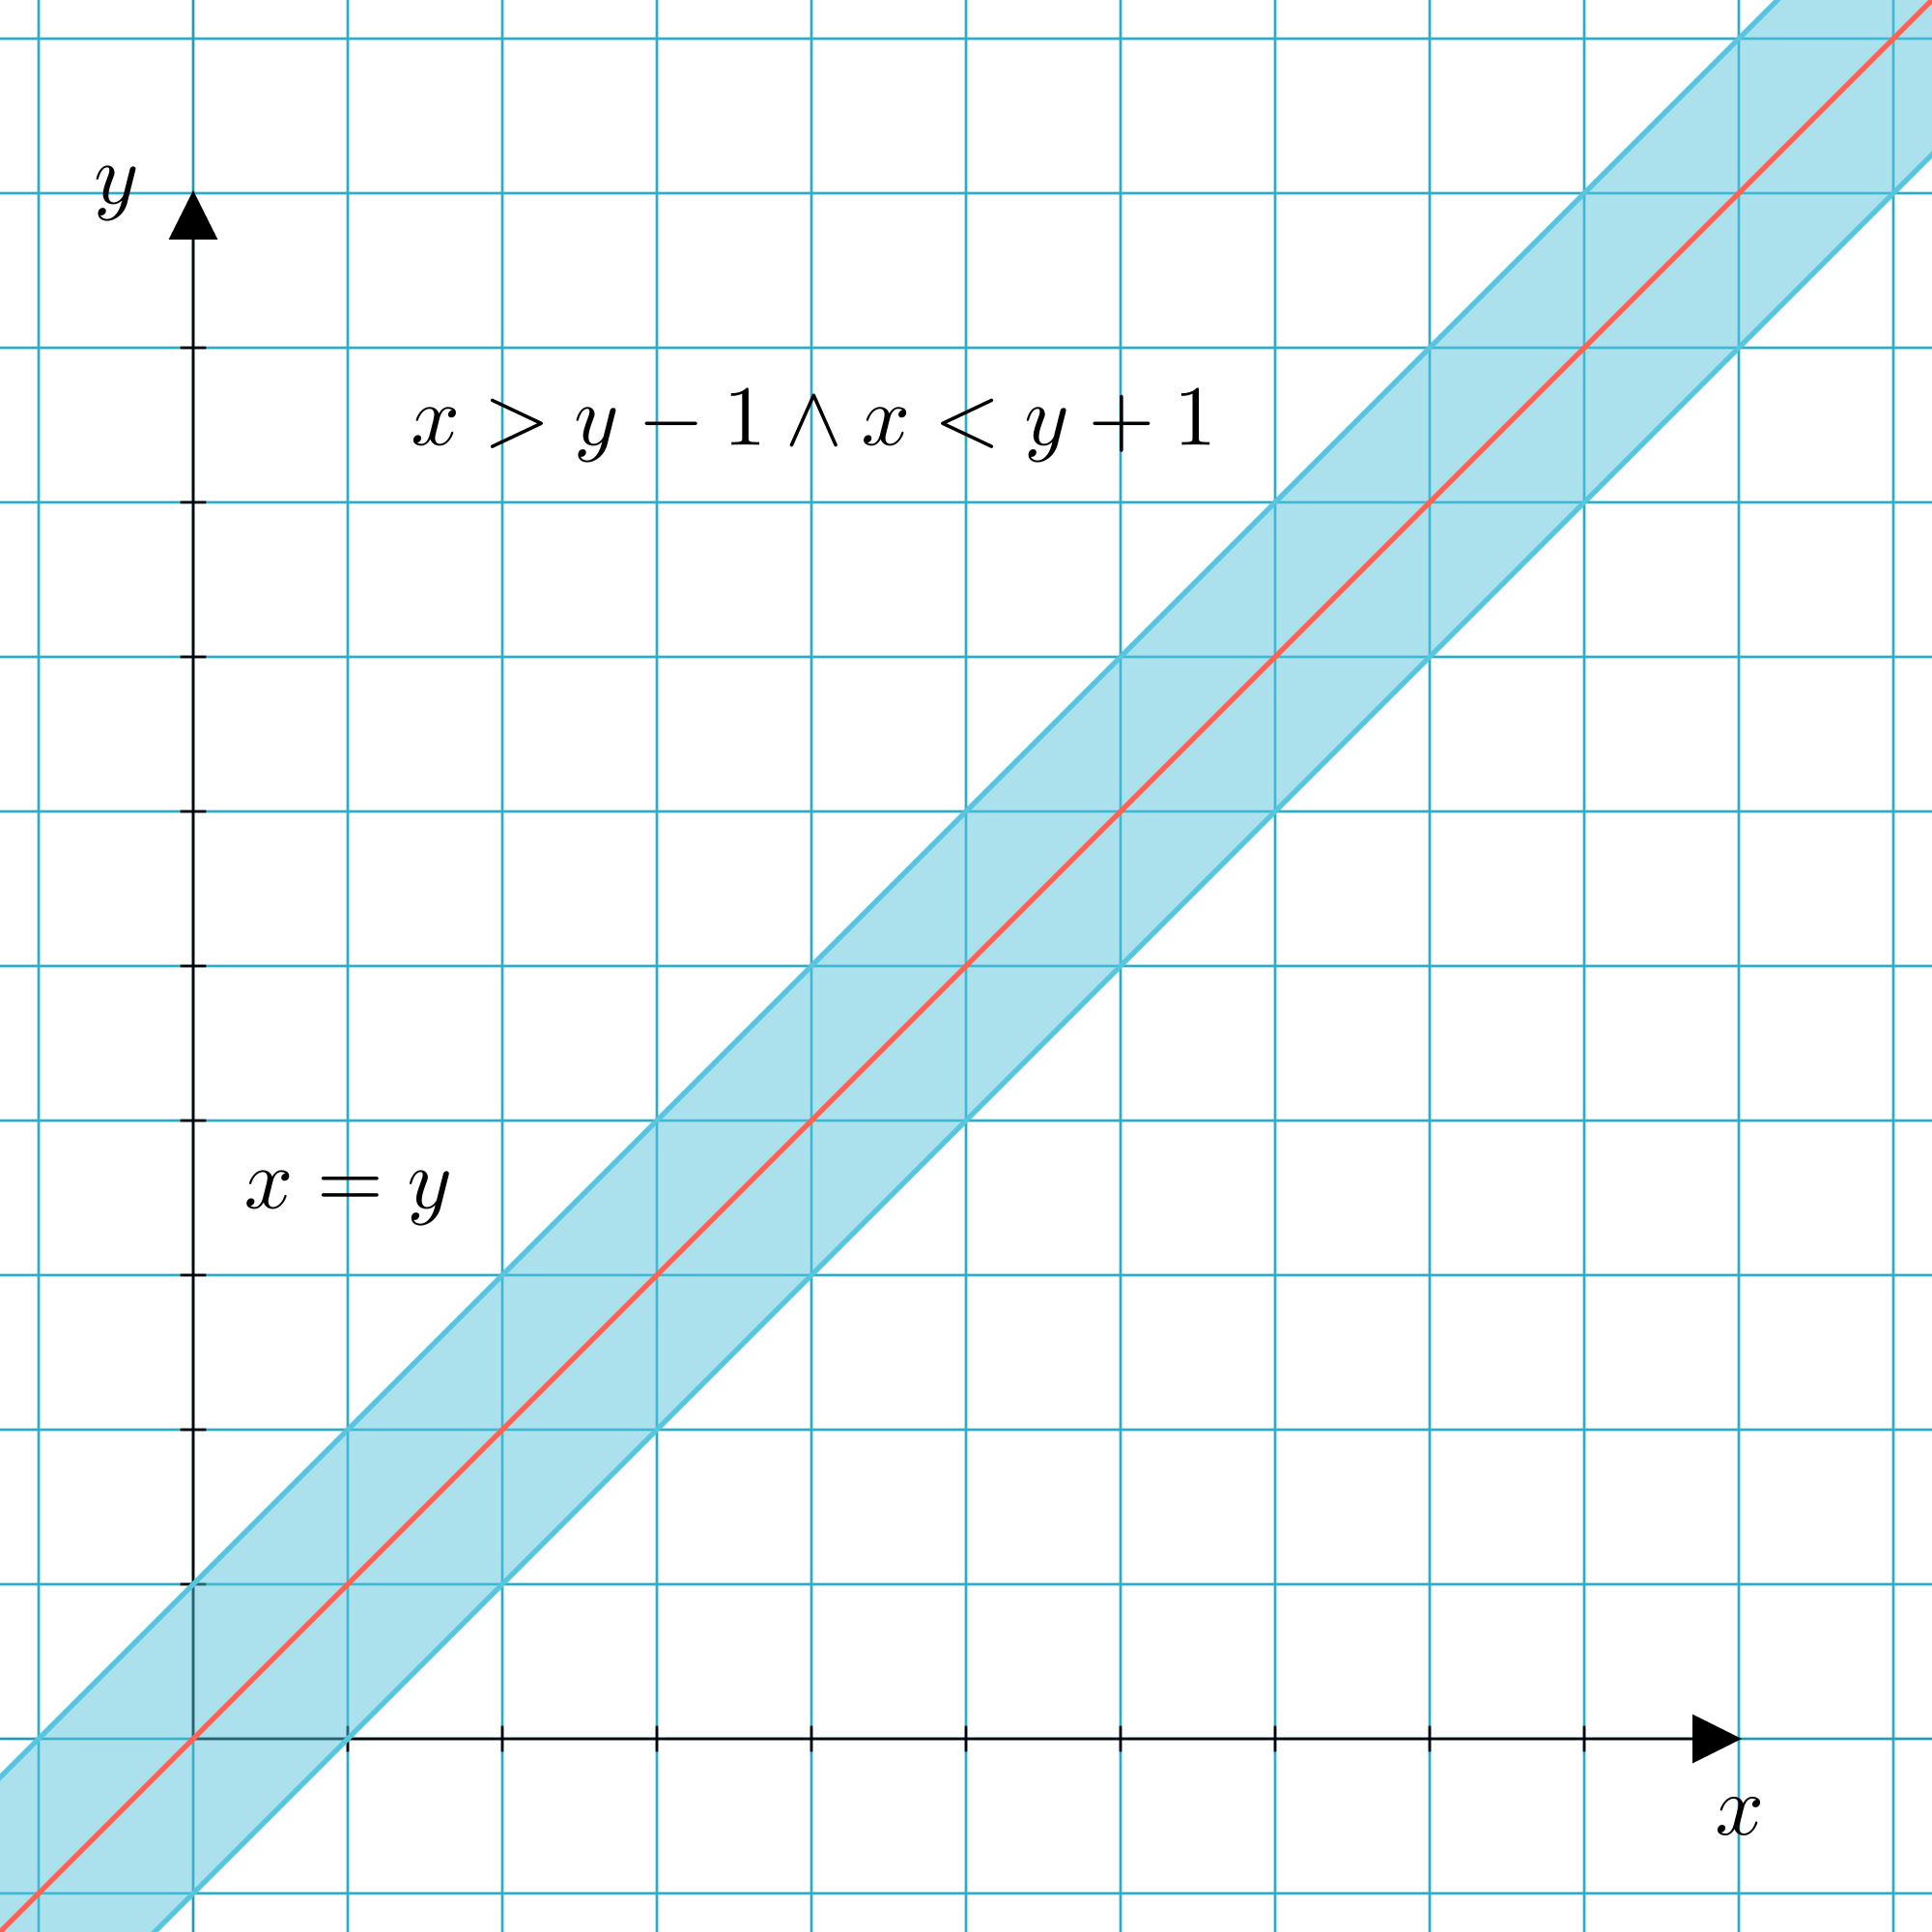
\includegraphics[width=0.5\linewidth]{../context-space.png}
	\caption{Figure showing a value space, where inclusion can not be shown}
	\label{fig:flux-context-space}
\end{figure}

The subtyping rules are quite similar. To the degree applicable, \textsc{S-Exists} is analogous to \textsc{$\preceq$-Ty}.

Another difference is the choice of target language: Flux chose $\lambda_{\text{Rust}}$ by Jung et al. \cite{jung_rustbelt_2018} as a basis for the formalization, which expresses the semantics in a continuation passing style over a language based on Rustc's MIR. 
On the other hand Corten based the formalization on a language based on Rustc's HIR and semantics expressed in a small-spec semantic. 

The corresponding implementations also use the MIR and HIR respectively. The advantages and disadvantages are discussed in \cref{ch:implementation}. Flux takes advantage of the MIR to cover a greater variety of control-flow scenarios.
Lehmann et al. also found, that "the refinement annotations [..] do not appear in Rust's MIR" \cite[p. 17]{lehmann_flux_2022}, which poses a challenge for the implementation.

Lastly Lehmann et al. evaluate Flux against Prusti proofing properties like "the absence of index-overflow error in a suite of vector-manipulating programs." \cite[p. 2]{lehmann_flux_2022}
Lehmann et al. found, that the liquid type inference system is powerful enough to infer necessary invariants for this use case, partly because "loop invariants express either simple inequalities or tedious bookkeeping" \cite[p. 21]{lehmann_flux_2022}
In these cases Prusti still required invariants to be specified, which Lehmann et al. party attribute to the fact, for every unchanged mutable reference, the invariant needs to state that the reference was not modified. By using \code{mut}, but not \code{strg} references, Flux could avoid that problem.
Even though Corten does not share the the strong references mechanism with Flux, the argument still applies: Corten would also not require additional invariants for the unchanging mutable references.
Because Corten does not support vectors (yet), a direct comparison is not possible.



\chapter{Conclusion \& Future Work} \label{ch:conclusion}

The goal of this thesis is to show, that Refinement Types can be idiomatically adapted to languages with unique mutable references. 
The thesis has show, that CortenC can type check Refinement Types in Rust, enforcing properties over mutable data and references and that these types fit idiomatically into Rust, if an inference system was added to CortenC.
The type system was sufficiently expressive for verifying complex properties about mutable data, recursive functions and loop invariants. 
In addition, the thesis analyzed the use of mutability in Rust and reaffirmed the limited prevalence of \code{unsafe} in Rust code.
For a subset of Rust (named Corten), a formal description of the syntax and small-step semantics was described.
A syntax for Refinement Types for Rust was devised and an accompanying type system was designed.
Based in the formal description, a proof-of-concept implementation shows, that automatic type checking of this type system is possible and feasible. The implementation also shows, that using the interface provided by Rustc is practical and beneficial for user-friendliness.

The evaluations has shown, that meaningful specifications can be automatically type checked. 
As planned and suspected, the lack of an inference system, calls for some avoidable specification, otherwise the evaluation has demonstrated, that the required specification effort is limited.
The breath of features implemented in the thesis is limited, mainly because getting the foundations right took some experimenting, though the foundations layed in the thesis are purposefully designed with these extensions in mind. Therefore covering more language features should be unproblematic.


In terms of future work, there are two axis to work on: 
On one hand covering more language features, like records or algebraic data types, would greatly improve the practicality of CortenC. 

On the other hand expanding the expressiveness of the type system would also be interesting: Introducing abstract predicates would allow a whole new set of properties to be specified. In particular developing a model of concurrency patterns could be a great application for them in Rust.

\fi

%% content

%% --------------------
%% |   Bibliography   |
%% --------------------

%% Add entry to the table of contents for the bibliography
\printbibliography[heading=bibintoc]

%% ----------------
%% |   Appendix   |
%% ----------------
\appendix


\begin{figure}[h]
	\centering
	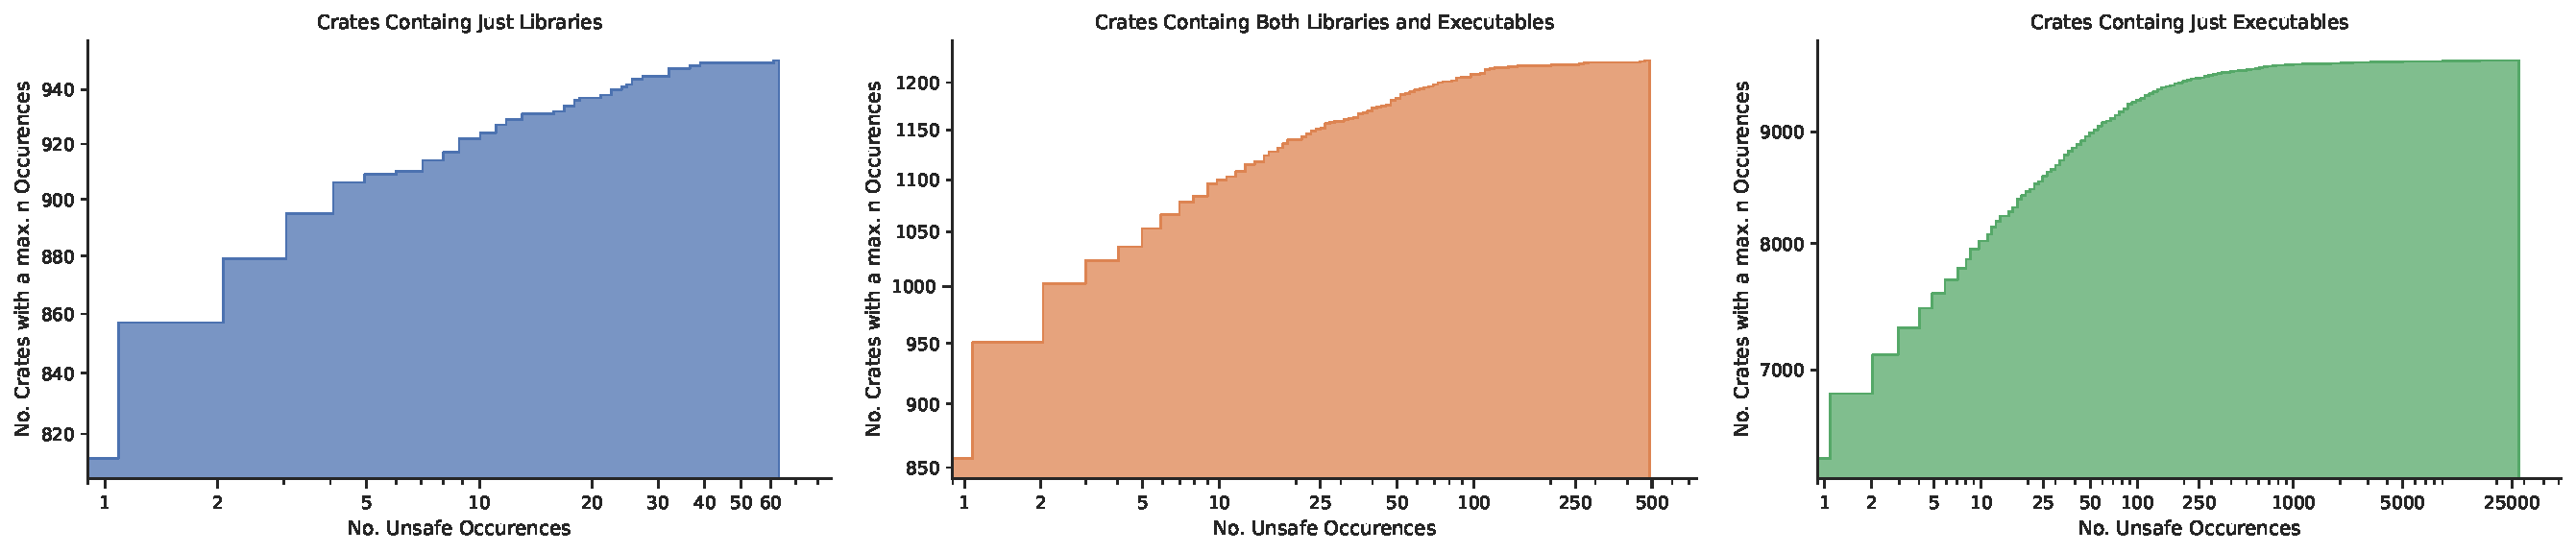
\includegraphics[width=0.99\linewidth, clip, trim={0.2cm 0.2cm 0.2cm 0.2cm}]{../unsafe-occurences-vs-no-crates.pdf}
	\caption{Cumulative, Logarithmic Histogram of the Amount of \code{unsafe} Uses in each Category}
	\label{fig:unsafe-hist}
\end{figure}


\begin{figure}[h]
	\centering
	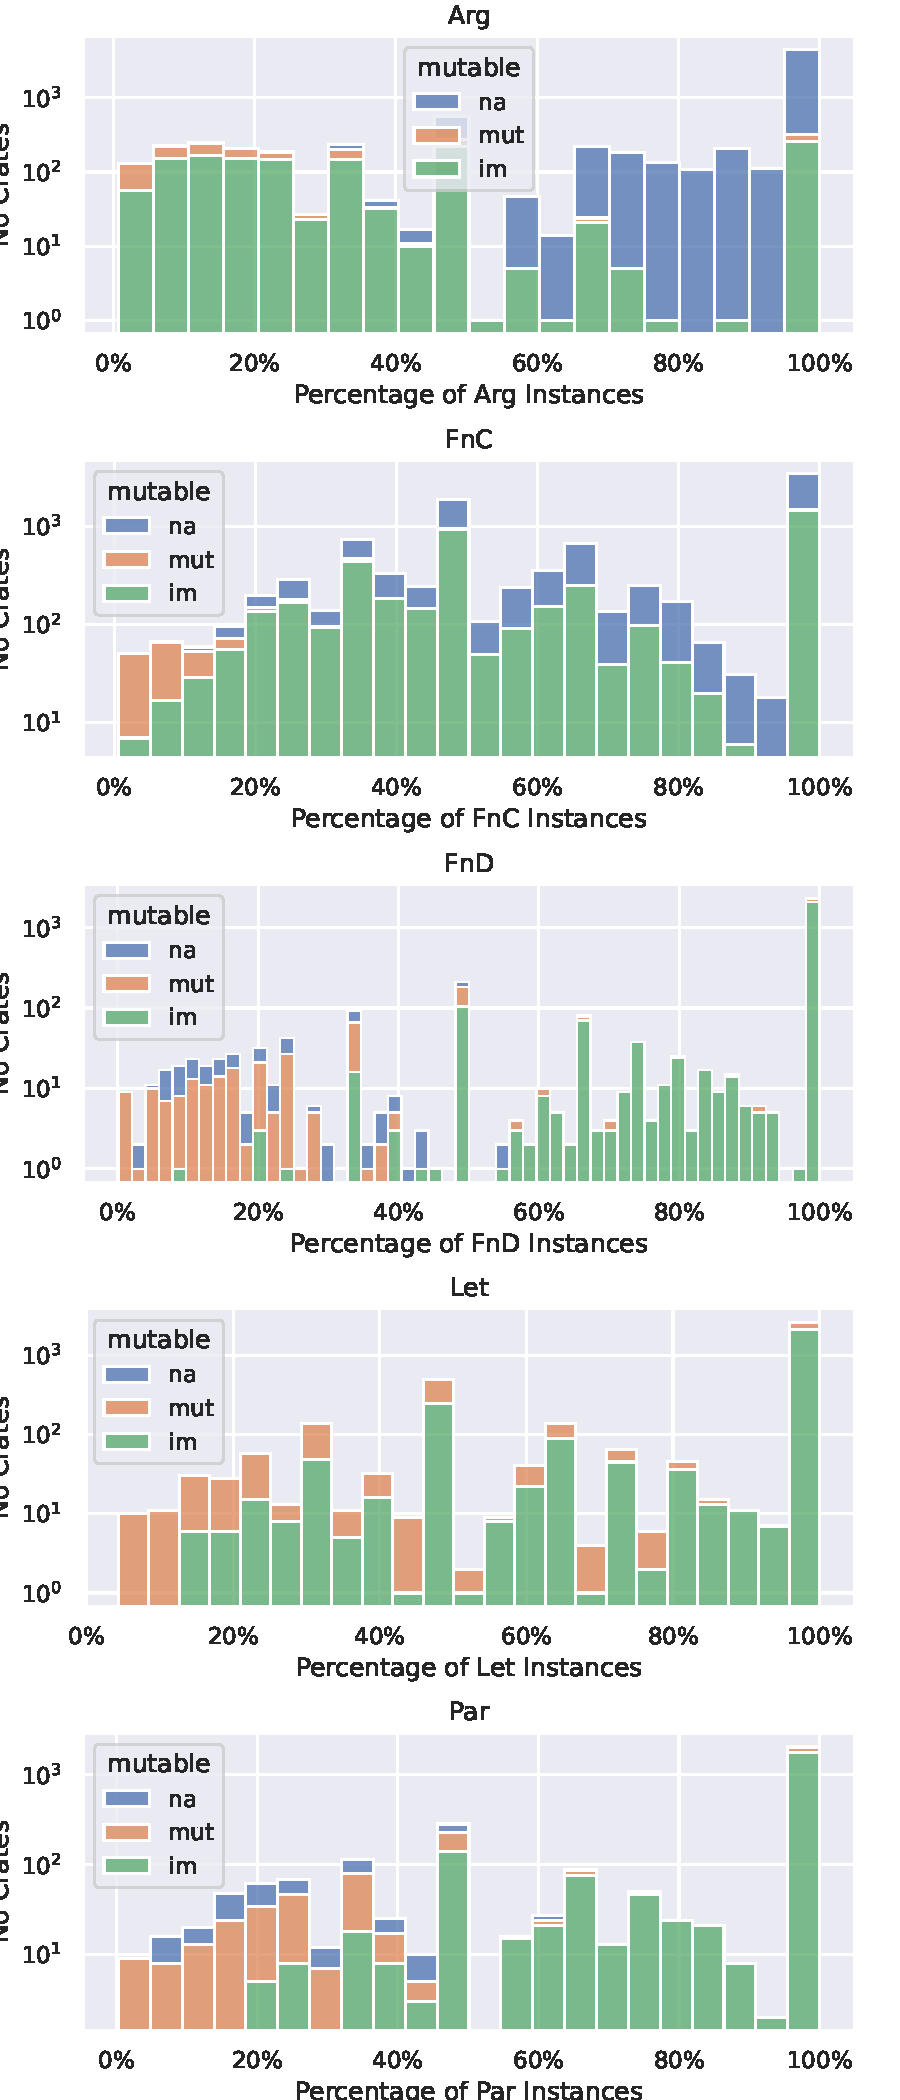
\includegraphics[width=0.99\linewidth, clip, trim={0.2cm 0.2cm 0.2cm 0.2cm}]{../hist-mutability.pdf}
	\caption{Logarithmic Histogram of the Number of Crates that contain n \% immutable / mutable items}
	\label{fig:mutability-hist}
\end{figure}

\end{document}
